% !BIB TS-program = biber

% -*- coding: utf-8 -*-
\documentclass{scrbook}[listof=totoc,listof=entryprefix,toc=chapterentrywithdots,headings=normal]% Entspricht den Typografieregeln eines Buches
\usepackage{wbh-thesis} % Laden der Vorlage
\usepackage{blindtext}
\usepackage{listings}
\usepackage[automark,headsepline]{scrlayer-scrpage}

\renewcommand{\lstlistingname}{Quelltext}% Listing -> Quelltext
\renewcommand{\lstlistlistingname}{Quellcodeverzeichnis}
\newcommand\listoflolentryname\lstlistingname

\usepackage{booktabs}
\usepackage{caption}
\usepackage[printonlyused]{acronym}
\usepackage{tabularx} 
\usepackage{hyperref}
\usepackage{xltabular}
\setlength{\extrarowheight}{4pt}



\newcommand{\cmark}{\ding{51}}%

\KOMAoptions{%
    headsepline=true,   % header line
    footsepline=false,          % footer line
    plainheadsepline=false, % activate header line for plain pages
    plainfootsepline=false} % activate footer line for plain pages

\usepackage{mathtools}

\usepackage[framemethod=tikz]{mdframed}
\counterwithout*{footnote}{chapter}

% Shorthands
\newcommand*\iffdef{\overset{\text{def}}{\iff}}
\DeclarePairedDelimiter\abs{\lvert}{\rvert}
\DeclarePairedDelimiter\norm{\lVert}{\rVert}

\definecolor{WBH}{RGB}{0, 94, 166}

% Theorem
\mdtheorem[
  linecolor=WBH,
  frametitlefont=\sffamily\bfseries\color{white},
  frametitlebackgroundcolor=WBH,
]{Def}{Defintion}


\definecolor{codegreen}{rgb}{0,0.6,0}
\definecolor{codegray}{rgb}{0.5,0.5,0.5}
\definecolor{codepurple}{rgb}{0.58,0,0.82}
\definecolor{backcolour}{rgb}{0.95,0.95,0.92}

\definecolor{listingDartDocCommentColor}{rgb}{0.0,0.5,0.0}
\definecolor{listingDartTodoColor}{rgb}{0.6,0.0,0.0}
\definecolor{listingDartKeywordColor}{rgb}{0.1,0.0,0.5}

\usepackage{tikz}
\def\checkmark{\tikz\fill[scale=0.4](0,.35) -- (.25,0) -- (1,.7) -- (.25,.15) -- cycle;} 

\lstloadlanguages{% Check Dokumentation for further languages ...
csh,
Java
}
\definecolor{maroon}{rgb}{0.5,0,0}
\definecolor{darkgreen}{rgb}{0,0.5,0}

\lstdefinestyle{Codestyle}{
    backgroundcolor=\color{backcolour},   
    commentstyle=\color{codegreen},
    keywordstyle=\color{magenta},
    numberstyle=\tiny\color{codegray},
    stringstyle=\color{codepurple},
    basicstyle=\ttfamily\footnotesize,
    breakatwhitespace=false,         
    breaklines=false,                 
    captionpos=b,                    
    keepspaces=false,     
    columns=fullflexible,            
    numbers=left,                    
    numbersep=5pt,                  
    showspaces=false,                
    showstringspaces=false,
    showtabs=false,                  
    tabsize=1
}



\lstdefinelanguage{XML}
{
  morestring=[b]",
  moredelim=[s][\bfseries\color{maroon}]{<}{\ },
  moredelim=[s][\bfseries\color{maroon}]{</}{>},
  moredelim=[l][\bfseries\color{maroon}]{/>},
  moredelim=[l][\bfseries\color{maroon}]{>},
  morecomment=[s]{<?}{?>},
  morecomment=[s]{<!--}{-->},
  commentstyle=\color{darkgreen},
  stringstyle=\color{blue},
  identifierstyle=\color{red}
}

\definecolor{dkgreen}{rgb}{0,0.6,0}
\definecolor{gray}{rgb}{0.5,0.5,0.5}
\definecolor{mauve}{rgb}{0.58,0,0.82}

\definecolor{codegreen}{rgb}{0,0.6,0}
\definecolor{codegray}{rgb}{0.5,0.5,0.5}
\definecolor{codepurple}{rgb}{0.58,0,0.82}
\definecolor{backcolour}{rgb}{0.95, 0.95, 0.96}

\lstdefinelanguage{Dart} {
	morekeywords={Widget,class, if,int?,num, String,var,library,get, set,String,int,num ,await, async,  @override, return, Scaffold, AppBar, AppBar, TextField, ElevatedButton, GestureDetector, Card, Column, Center, Text, TextStyle,  MaterialApp,  extends, BuildContext, Tab, TabBarView, Icon, TabBar, with, InputDecoration, double, Map, bool,  List, import ,as, Future, void} ,
 	 morecomment=[l]{//},
	keywordstyle=\color{bluekeywords},
	commentstyle=\color{dkgreen}, 
	stringstyle=\color{mauve},
	numberstyle=\tiny\color{gray},
  	breaklines={true},
}


\definecolor{bluekeywords}{rgb}{0,0,1}
\definecolor{greencomments}{rgb}{0,0.5,0}
\definecolor{redstrings}{rgb}{0.64,0.08,0.08}
\definecolor{xmlcomments}{rgb}{0.5,0.5,0.5}
\definecolor{types}{rgb}{0.17,0.57,0.68}

\lstdefinelanguage{csh} {
morekeywords={ abstract, event, new, struct, as, explicit, null, switch,base, extern, object, this,bool, false, operator, throw,break, finally, out, true,byte, fixed, override, try,case, float, params, typeof,catch, for, private, uint,char, foreach, protected, ulong,checked, goto, public, unchecked,class, if, readonly, unsafe,const, implicit, ref, ushort,continue, in, return, using,decimal, int, async, await,sbyte, virtual,default, interface, sealed, volatile,delegate, internal, short, void,do, is,sizeof, while,double, lock, stackalloc,else, long, static, enum, namespace, List, EventArgs,string, Dictionary, Assert, Task, String},
commentstyle=\color{greencomments},
morekeywords={partial, var, value, get, set},
keywordstyle=\color{bluekeywords},
morecomment=[l]{//},
stringstyle=\color{redstrings},
}
\usepackage{ltxtable}



\lstset{style=Codestyle}

\usepackage{microtype}
\pagestyle{scrheadings}

\setlength{\headheight}{18pt}
\setlength{\footheight}{18pt}

\clearscrheadfoot

\ihead{\leftmark}
\ohead{\pagemark} 
\renewcommand*{\chapterpagestyle}{scrheadings}

\hyphenation{
platt-form-spe-zi-fi-schen
Code-erzeugung
Ereignis-erkennung
Re-prä-sen-ta-ti-on-en
Benutzer-ober-fläche
Benutzer-erlebnis
}

\setcounter{biburllcpenalty}{7000}
\setcounter{biburlucpenalty}{8000}
\KOMAoptions{listof=graduated}% das automatische listof=flat von
                              % listof=entryprefix wieder deaktivieren (siehe
                              % KOMA-Script-Anleitug)
\DeclareTOCStyleEntries[indent=0pt,numwidth=1cm,level=1]{tocline}{figure,table,lstlisting}% Alle Einträge auf Stil tocline mit den angegebenen Einstellungen ändern. Zu der Bedeutung aller Optionen siehe die KOMA-Script-Anleitung.


\newcommand{\Csharp}{%
  {\settoheight{\dimen0}{C}C\kern-.05em \resizebox{!}{\dimen0}{\raisebox{\depth}{\#}}}}


  \begin{document}

  \begin{titlepage}
\begin{center}
\newcommand{\HRule}{\rule{.9\linewidth}{.6pt}} % New command to make the lines in the title page

\vspace*{.06\textheight}
{\scshape\LARGE Wilhelm Büchner Hochschule}\vspace{1.5cm} % University name
\textsc{\Large Masterthesis}\\[0.5cm] % Thesis type

\HRule \\[0.4cm] % Horizontal line
{\huge \bfseries Realisierung eines Source-to-Source Compilers zwischen Xamarin.Forms und Flutter zur automatisierten Transformation bestehender mobiler Anwendungen}\vspace{0.4cm} % Thesis title
\HRule \\[1.5cm] % Horizontal line
 
\begin{minipage}[t]{0.4\textwidth}
\begin{flushleft} \large
\emph{Author:}\\
Julian Pasqué % Author name - remove the \href bracket to remove the link
\end{flushleft}
\end{minipage}
\begin{minipage}[t]{0.4\textwidth}
\begin{flushright} \large
\emph{Betreuer:} \\
Dr. Thomas Kalbe % Supervisor name - remove the \href bracket to remove the link  
\end{flushright}
\end{minipage}\\[3cm]
 
\vfill


\large Masterstudiengang  Verteilte und mobile Anwendungen\\[0.8cm] % Research group name and department name
\large Fachbereich Informatik\\[0.8cm] % Research group name and department name
\large Matrikelnummer: 902953 \\[0.8cm] % Research group name and department name
 
\vfill

{\large \today}\\[6cm] % Date
 
\vfill
\end{center}
\end{titlepage}  % Setzt die Titelseite
  \frontmatter        % Eigenschaften für den Vorspann setzen
  \renewcommand*\chapterheadstartvskip{}% removes space before chapter titles 

  \include{Abstract}  % Setzt die Titelseite

  \tableofcontents    % Setzt das Inhaltsverzeichnis
  \listoffigures      % Setzt das Abbildungsverzeichnis
  
  \listoftables       % Setzt das Tabellenverzeichnis
  \include{Abkürzungsverzeichnis}

  \let\footnotemark\relax
  \lstlistoflistings

  \mainmatter         % Eigenschaften für den Hauptteil setzen
  \KOMAoptions{headings=big}% restores default space before chapter titles

  \renewcommand*{\chapterpagestyle}{plain}
  %%% bitte die nächsten 5 Zeilen löschen
\chapter{Einleitung}
Durch die Entwicklung von verschiedenen mobilen Geräten mit unterschiedlichsten Hardwarekomponenten und Betriebssystemen hat sich ein stark fragmentierter Markt ergeben.\footcite[Vgl.][S. 3]{Joorabchi2016}  Diese Marktentwicklung hat einen direkten Einfluss auf die Softwareentwicklung für mobile Endgeräte und damit zu der Entwicklung von Cross-Plattform Frameworks wie Xamarin.Forms und Flutter gesorgt. Durch die Abstraktion von Hardware und Betriebssystem bieten diese Frameworks die Möglichkeit Anwendungen für die verschiedenen Plattformen mit einer gemeinsamen Quelltextbasis zu entwickeln und somit Kosten und Zeit zu sparen. \footcite[Vgl.][S. 295]{Vollmer2017} 
Der Möglichkeit Entwicklungsressourcen zu sparen steht das Risiko der Abhängigkeit entgegen, da sich alle Frameworks zur Cross-Plattform-Programmierung in den verwendeten Programmiersprachen sowie ihrer Arbeitsweise unterscheiden, ist ein Wechsel zwischen den einzelnen alternativen mit enormen Arbeitsaufwenden verbunden. \footcite[Vgl.][S. 64]{Wissel2017}  
\section{Ziel der Arbeit}
Im Rahmen dieser Arbeit soll ein Source-To-Source Compiler zwischen den Frameworks Xamarin.Forms und Flutter realisiert werden mit dessen Hilfe die folgende zentrale Forschungsfrage beantwortet werden soll: "Können Apps komplett automatisiert von Xamarin.Forms zu Flutter übersetzt werden, oder sind manuelle Arbeitsschritte erforderlich?"
\section{Motivation}
Im Mai 2020 hat Microsoft mit .NET MAUI einen Nachfolger für das Xamarin.Forms Framework angekündigt, der im Herbst 2021 zusammen mit der sechsten Version des .NET Frameworks veröffentlicht werden soll. Zum aktuellen Zeitpunkt ist bereits angekündigt, dass .NET MAUI grundlegende Änderung mit sich bringt und Anwendungen die mit Hilfe von Xamarin.Forms entwickelt wurden angepasst werden müssen.\footcite[Vgl.][Abgerufen am 28.10.2020]{Hunter2020}

Für Xamarin.Forms Entwickler wird es also unausweichlich sein, grundlegende Änderungen an bereits realisierten Anwendungen vorzunehmen um in der Zukunft von Aktualisierungen zu profitieren. Aus diesem Grund eignet sich die Zeit, um auch alternative Frameworks zu analysieren und zu überprüfen ob ein  Umstieg lohnenswert ist. Das Flutter Framework erfreut sich unter Entwicklern einer wachsenden Beliebtheit und ist nicht nur auf Grund seiner performanten Anwendungen mittlerweile weit verbreitet. 

Ein automatisierter Umstieg auf das von Google entwickelte Framework würde also nicht nur die Anpassungen an .NET Maui verhindern, sondern auch leistungsfähigere Anwendungen generieren. 

\section{Gliederrung}

  \chapter{Compiler}


Programmiersprachen dienen als Verständigungsmittel zwischen Programmierern und Rechenanlagen. Diese Sprachen haben sich in der Vergangenheit dabei immer mehr an die  Terminologie eines bestimmtes Anwendungsgebietes angenähert. Durch diese Entwicklung eigneten sich Programmiersprachen direkt für die Dokumentation von entwickelten Algorithmen und Anwendungen, entfernten sich jedoch weiter von den Gegebenheiten des realen Rechners.\footcite[Vgl.][S. 15]{Schneider1975}
\begin{figure}[h]
 \includegraphics[width=\textwidth,height=\textheight,keepaspectratio]{Images/LanguageIntermediary.png}
 \caption{Programmiersprachen als Schnittstelle}
 \label{fig:Programmiersprachen als Schnittstelle}
\end{figure}
Für die Ausführung einer in einer problemorientierten Programmiersprache geschriebenen Anwendung ist es notwendig, die Sprache in eine maschinenorientierte Form zu überführen. \footcite[Vgl.][S. 15]{Schneider1975} Bereits im Jahre 1952 stelle Rutishauser fest,  dass Computer in der Lage sind diesen Übersetzungsvorgang selbst durchzuführen.\footcite[Vgl.][S. 312]{Rutishauser1952} 
Durch die Möglichkeit zur automatischen Übersetzung von problemorientierten Programmiersprachen konnten Hochsprachen entwickelt werden, die menschenfreundliche Sprachelemente anstatt Maschineninstruktionen verwenden. \footcite[Vgl.][S. 47]{Wagenknecht2014}
\section{ Grundbegriffe}
Diese historische Einführung zeigt,  dass Software zur automatisierten Übersetzung schon seit der Mitte des letzten Jahrhunderts thematisiert wurde, so hat sich in der Wissenschaft eine einheitliche Definition ergeben.  \citeauthor{Ullmann2008} beschreibt die sogenannten Compiler im Jahre \citeyear{Ullmann2008} wie folgt:\footcite[Vgl.][S. 1]{Ullmann2008} 
\begin{Def}[Compiler]
Ein Compiler ist ein Programm, welches ein anderes Programm aus einer Quellsprache in ein gleichwertiges Programm einer Zielsprache übersetzen kann.
\end{Def} 
\vspace{-1em}

Aus dieser Definition lässt sich ein für diese Arbeit relevanter Fakt ableiten: Compiler sind nicht ausschließlich Übersetzer zwischen zwischen problemorientierten,- und maschinenorientierten Programmiersprachen.  Sie sind ausschließlich für die Übersetzung von einer Quellsprache in eine Zielsprache verantwortlich.  Auch wenn der Begriff Programm für jedermann geläufig ist,  kann es dennoch passieren,  das von verschiedenen Repräsentationen eines Programmes gesprochen wird.  So können alle drei der folgenden Begriffe als Programm bezeichnet werden: Der Quelltext, dass ausführbare Programm kann er dennoch unterschiedliche Repräsentationen eines Programmes meinen.  Für das weitere Verständnis dieser Arbeit ist,  mit dem Begriff Programm die ausführbare Anwendung auf den Smartphones des Anwenders gemeint.  

Neben der Übersetzung von problem zu maschinenorientierter Sprache gibt es ebenfalls Compiler, die andere Ziele verfolgen. Dazu gehört zum Beispiel die sogenannten Binärübersetzer,  die den Binärcode eines Programmes für andere Rechner übersetzen, sodass er auf diesen ausgeführt werden kann.  \footcite[Vgl.][S. 27]{Ullmann2008} Ein Source-to-Source(S2S) Compiler,  häufig auch als "Transpiler" bezeichnet,  ist ebenfalls eine besondere Ausprägung eines Compilers die sich wie folgt definieren lässt.  \footcite[Vgl.][S. 1629]{IJCSIT2015}
\begin{Def}[Source-to-Source Compiler]
Ein Source-to-Source-Compiler ist ein Compiler, bei dem sowohl die Quellsprache als auch die Zielsprache eine Hochsprache ist.
\end{Def}
\vspace{-1em}

Der Begriff Hochsprache ist dabei ein Synonym für die bereits eingeführten problemnahen Sprachen wie zum Beispiel C++,  Java,  C\# oder Dart und damit für den Menschen in einer lesbaren und änderbaren Form geschrieben sind. \footcite[Vgl.][S. 9]{Eisenecker2008} 



\subsection{ Syntax und Semantik}
Die Syntax einer Programmiersprache ist das Aussehen bzw. die Struktur des Quelltextes. Der komplette Quelltext eines Programms muss syntaktisch korrekt sein, damit er übersetzt werden kann.  \\
Die Semantik ist die Bedeutung, die den verschiedenen syntaktischen Strukturen zugeordnet werden kann. Es ist also von der Semantik abhängig auf welche Art und Weise die Weiterverabeitung durch den Compiler erfolgt. 




\section{Aufgabe}
Die Aufgaben des Compilers lassen sich, mit dem Ziel der Übersetzung von Programmiersprachen, in die zwei Unteraufgaben Analyse und Synthese unterteilen. \footcite[Vgl.][S. 6]{Ullmann2008}\\
Bei der Analyse wird das Programm in seine Bestandteile zerlegt und mit einer grammatischen Struktur versehen. Diese wird anschließend verwendet um eine Zwischendarstellung des Quellprogramms zu erstellen. Dabei wird überprüft, ob das Programm syntaktisch oder semantisch nicht wohlgeformt ist, und ob der Programmierer Änderungen vornehmen muss. Außerdem werden bei der Analyse Informationen über das Quellprogramm gesammelt und in einer so genannten Symboltabelle abgelegt.  \footcite[Vgl.][S. 6f]{Ullmann2008}\\
Bei der Synthese wird aus der Zwischendarstellung un den Informationen aus der Symboltabelle das gewünschte Zielprogramm konstruiert. Der Teil des Compilers, der sich mit der Analyse befasst wird oft als Front-End bezeichnet, derjenige der für die Synthese zustädnig ist als Back-End.  \footcite[Vgl.][S. 7]{Ullmann2008}
\section{Phasen}
Der Vorgang des Kompilieren lässt sich nach \citeauthor{Ullmann2008} in mehere Phasen unterteilen, die an dieser Stelle eingeführt werden sollen. \footcite[Vgl.][S. 6]{Ullmann2008}
\subsection{Lexikalische Analyse}
Die erste Phase eines Compilers ist die sogenannte lexikalische Analyse. Dabei wird der Zeichenstream, der das Quellprogramm bildet in Lexeme gegliedert. Für jedes erzeugte Lexem gibt der lexikalische analysator ein Token in folgender Form aus:\footcite[Vgl.][S. 7f]{Ullmann2008}
\begin{center}
 <Name, Attributwert>
\end{center}
Der Name ist dabei ein abstaktes Symbol, das während der nächste Phase, der Syntaxanalyse verwendet wird. Der Attributwert auf einen Eintrag in der symboltabelle für dieses Token zeigt. Diese Informationen werden in den späteren Phasen für die semantische Analyse und die Codegeneriung benötigt. \footcite[Vgl.][S. 7f]{Ullmann2008}
\subsection{Syntaxanalyse}
Die zweite Phase des Compilers ist die Syntaxanalye. Dafür verwendet der sogenannte Parser die vom lexikalischen Analysator ausgegebenen Token um eine baumartige Zwischendarstellung zu erstellen. die die grammatische Struktur der Tokens zeigt. Die Darstellung wird daher auch häufig als Syntaxbaum bezeichnet. Die Knoten stehen dabei für eine Operation und seine Kindknoten für die Argumente dieser Operation. Die Anordnung er Operationen stimmt mit üblichen arithmentischen Konventionen überein, wie zum Beispiel der vorrang der Multiplikation vor Addition. \footcite[Vgl.][S. 9]{Ullmann2008}
\subsection{Semantische Analyse}
Bei der semantischen Analyse wird der Syntaxbaum und die Informationen aus der Symboltabelle verwendet um das Quellprogramm auf semantische Konsistenz mit der Sprachdefinition zu überprüfen. Außerdem werden in dieser Typinformationen gesammelt und entweder im Syntaxbaum oder in der Symboltabelle hinterlegt um sie in späteren Phasen zu verwenden. Dabei werden außerdem Typen überprüft, daher analysiert ob jeder Operator die passenden Operanden hat. \footcite[Vgl.][S. 9ff]{Ullmann2008}
\subsection{Zwischencodeerzeugung}
Bei der Übersetzung eines Quellprogramms in den Zielcode kann der Compiler mehrere Zwischendarstellungen in verschiedenen Formen erstellen. Syntaxbäume sind beispielsweise eine solche Darstellung. Nach der semantischen Analyse stellen viele Compiler eine maschinennahe Zwischendarstellung die für eine Abstrakte Maschine entworfen wurden.  \footcite[Vgl.][S. 11]{Ullmann2008}
\subsection{Codeoptimierung}
In dieser Phase wird der maschinenunabhängige Code so optimiert, dass sich darauf ein besserer Zielcode ergibt. Dabei bedeutet besser, schnellerer code oder code der weniger Ressourcen verbraucht. Der Umfang der Codeoptimierung schwankt dabei von Compiler zu Compiler erheblich.  \footcite[Vgl.][S. 11f]{Ullmann2008}
\subsection{Codeerzeugung}
Bei der Codeerzegung werden die Eingaben aus der Zwischendarstellung des Quellprogramms entgegengenommen und auf die Zielsprache abgebildet. Ein entsheidender Aspekt der Codeerzeugung ist die sinnvolle zuweisung von Registern für Variablen, falls es sich bei der Zielsprache um Maschinencode handelt.\footcite[Vgl.][S. 13]{Ullmann2008}

\section{Rekursiver Ansatz}
  \chapter{Compiler Entwurf}
Basierend auf der theoretischen Einführung von Compilern kann nun ein Entwurf für den Source to Source Compilers erstellt werden auf dessen Basis in späteren Kapiteln eben dieser Implementiert werden soll.  Die Phasen aus dem vorherigen Kapiteln sollen in dem in dieser dieser Arbeit zu entwickelnden Übersetzers ebenfalls durchlaufen werden.  
Wie bereits in der Definition zu Compilern aufgeführt,  muss das Ziel des Compilers sein eine gleichwertige mobile Anwendung zur Verfügung zu stellen.  Im Falle dieses Compilers bedeutet dies,  dass die resultierende Flutter App sich identisch wie die ausgehende Xamarin.Forms App verhalten sollte.  Da es sich bei beiden Frameworks um große ausgereifte Open Source Projekte handelt,  hat sich um die Frameworks eine Vielzahl von Erweiterungen in Form von Plugins entwickelt.  Da es sich bei diesen Erweiterungen nicht zwangsläufig um Open-Source Projekte handelt hat der zu entwickelnde Übersetzer keinen Zugriff auf den Quelltext und kann diesen daher nicht Übersetzen.  Der Einfachheit halber soll der in dieser Arbeit entwickelte Prototyp ausschließlich Elemente die im Eigentlichen Framework Xamarin.Forms vorhanden sind sowie die Inhalte des Optional Verfügbaren Packetes Xamarin.Essentials, welches ebenfalls von Microsoft ist übersetzen. 

\section{Struktur}

Xamarin.Forms Quelltext-Dokumente lassen sich in zwei Kategorien unterteilen.  Den XAML (Extensible Application Markup Language) Dateien,  die eine Benutzeroberfläche beschreiben,  sowie den CS- Dateien welche den C\# Quelltext beinhalten.  Bei Dateien mit der Endung XAML.CS  handelt es sich um Quelltext Dokumente,  die die Logik für eine Ansicht beschreiben.  Für die Übersetzung der Anwendung hat dies eine besondere Bedeutung,  da XAML und XAML.CS Dateien zusammen eine Ansicht und ihr Verhalten definieren.  Alleinstehende .CS Dateien beschreiben die anderen Klassen der Anwendung und können unabhängig betrachtet werden.  Abbildung \ref{fig:CompilerStruktur} zeigt die Struktur des zu realisierenden Übersetzers auf einer hohen Abstraktionsebene.
\begin{figure}[!ht]
 \includegraphics[width=14.5cm,height=5.3cm]{Images/Compiler/CompilerArchitecture.png}
 \caption{Compiler Struktur}
 \label{fig:}
\end{figure}

Wie man in der Abbildung sehen kann unterteilt sich die Übersetzung zwischen Dateien mit generellen Klassendefinition und jeweils zwei Dateien für Ansichten.  Für das Framework Flutter,  in welches diese Dateien überführt werden sollen gibt es nur eine Art von Dateien mit der Dateiendung Dart.
Im folgenden soll jeweils erläutert werden, wie die Dateien von Ansichten und generelle C\# Klassen übersetzt werden sollen.  Durch eine Kombination von beiden Teilen sollte anschließend eine gleichwertige mobile Anwendung ergeben. 

\subsection{Dateien für die Anzeige }
\subsection{Generelle C\# Klassen}



\section{Rosyln als Ausgangssituation}
Wichtig für den Entwurf ist die Erkenntnis,  dass der modulare C\# Compiler Roslyn als Einstiegspunkt für die Übersetzung verwendet werden kann.  So kann auf eine ausgereifte Plattform für die ersten Phasen der Compilierung zurückgegriffen werden.




\section{Code optimierung}
Die Code Optimierung ist der essentielle Teil der Übersetzung.  Beide Frameworks arbeiten grundlegend Unterschiedlich,  sodass eine einfache Übersetzung nicht zu einer funktionsfähigen Anwendung führen würde.  Daher ist es notwendig,  beide Frameworks zu analysieren und die genauen Unterschiede zwischen den Arbeitsweisen zu verstehend. Anschließend muss bei der Übersetzung darauf geachtet werden,  die Xamarin.Forms Anwendung in eine Form zu überführen bei der Sie in Form einer Flutter App auf sowohl iOS als auch Android ausgeführt werden kann.   
  \chapter{Technische Unterschiede zwischen Xamarin.Forms und Flutter}
\label{chap:CrossPlattformFrameworks}

Die Unterschiede zwischen den Frameworks werden im folgenden genauer betrachtet.  Für den technischen Vergleich dient Xamarin.Forms als Grundlage.  Die Namen von Abschnitten und Unterabschnitten orientieren sich deshalb an dessen Terminologie.  In den jeweiligen Gliederungspunkten wird anschließend genauer betrachtet,  wie sich spezielle Arbeitsweisen oder Darstellungsoptionen in Flutter abbilden lassen. 

\section{Projektaufbau}
Xamarin.Forms weißt eine andere Projektstruktur auf als Flutter,  das nur mit einem Projekt arbeitet.  Wärend das Flutter Projekt alle notwendigen Inhalte für iOS und Android inkludiert, \footcite[Vgl.][S. 113]{Biessek2019} setzt sich die Projektmappe bei Xamarin.Forms aus mehreren Projekten zusammen.  Es gibt für jede Plattform ein dediziertes Projekt, dass den plattformspezifischen Code,  Konfigurationen und Icons beinhaltet, sowie ein Projekt für den plattformunabhängigen Quelltext.   \footcite[Vgl.][S. 25f.]{Petzold2016} Icons und Konfigurationen werden bei Flutter in einem gleichen oder ähnlichen Format und nur in einem anderen Projekt hinterlegt und lassen sich folglich migrieren.  In den Ausschlusskriterien in Kapitel \ref{chap:CompilerEntwurf} dieser Arbeit wurde bereits der plattformspezifische Quelltext von Xamarin.Forms für die Übersetzung exkludiert.  
\section{Ansichten}
Ansichten (engl. Views) sind visuelle Elemente, die in zwei Kategorien unterschieden werden können.  Steuerelemente (engl. Controls) sind für die Sammlung von Benutzereingaben oder die Ausgabe von Daten verantwortlich und Layouts, beinhalten eine Sammlung von Ansichten und sind für ihre visuelle Anordung auf der Benutzeroberfläche verantwortlich.  \footcite[Vgl.][Abgerufen am \today]{Ritscher2020}

\subsection{Layouts}
Ähnlich wie die Ansichten lassen sich auch die Layouts in zwei Kategorien unterteilen.  Den Ansichtsseiten (engl. Pages) sowie den generellen Layouts. 
Die Pages nehmen den gesamten Bildschirm ein und werden in Abbildung \ref{fig:Xamarin.Forms Pages} dargestellt.\footcite[Vgl.][Abgerufen am \today]{MicrosoftXamPages2016}  

\begin{figure}[!ht]
 \includegraphics[width=\textwidth,height=\textheight,keepaspectratio]{Images/CrossPlattformFrameworks/XamarinFormsPages.png}
 \caption[Xamarin.Forms Pages]{Xamarin.Forms Pages\footcite{MicrosoftXamPages2016}}
 \label{fig:Xamarin.Forms Pages}
\end{figure}

\glq ContentPage\grq{} ist ausschließlich für die Anzeige einer weiteren Ansicht verantwortlich.  Die drei anderen Pages besitzen ein Navigationskonzept.  \footcitetext[Abbildung in Anlehnung an][Abgerufen am \today]{MicrosoftXamPages2016} \glq FlyOutPage\grq{} teilt den Bildschirm in zwei Bereiche, ein Bereich dient der Navigation.  Er enthält ein Menü das, wie im Namen enthalten, einfliegen kann.  Der zweite Bereich zeigt eine Detailansicht,  in welcher der Inhalt der angeforderten Seite geladen wird.  \glq NavigationPage\grq{} bietet eine Navigationsleiste, die einen Titel der aktuellen Seite und eine Navigationsschaltfläche beinhalten kann.  \glq TabbedPage\grq{} stellt die unterschiedlichen Seiten als Registerkarten dar. \footcite[Vgl.][Abgerufen am \today]{MicrosoftXamPages2016}
Die Ansichtsseiten befinden sich in der Regel, innerhalb der \ac{xaml}-Datei, auf der untersten Ebene, dem so genannten Wurzelknoten. Der Quelltext \ref{lst:TabbedPage} zeigt dies exemplarisch für eine \glq TabbedPage\grq{} dargestellt,  angegeben.  

\lstinputlisting[label={lst:TabbedPage},caption={[Xamarin.Forms \glq TabbedPage\grq{} Definition]{Xamarin.Forms \glq TabbedPage\grq{} Definition\footcite[Quelltext in Anlehnung an][Abgerufen am \today]{MicrosoftXamTabbedView2020}}} , language=XML]{SourceCode/XamarinFormsTabbedPage.XAML}

\footcitetext[Quelltext in Anlehnung an][Abgerufen am \today]{MicrosoftXamTabbedView2020}Es wird eine \glq TabbedPage\grq{} mit drei Registerkarten entworfen.  Eine Kombination mehrerer Navigationskonzepte ist  möglich,  das Beispiel zeigt eine Navigationsleiste innerhalb der Registerkarten. 

Die verfügbaren Eigenschaften der Ansichtsseiten unterscheiden sich je nach Einsatzszenario.  Im folgenden Quelltext \ref{lst:FlyOutPage} wird dies exemplarisch an der Realisierung einer \glq FlyoutPage\grq{} deutlich.  Anders als bei \glq TabbedPage\grq{}, die aus einer Sammlung von Registerkarten besteht, finden sich im Quelltext die Eigenschaften \glq Flyout\grq{}  und \glq Detail\grq{}.

\lstinputlisting[label={lst:FlyOutPage}, caption={[Xamarin.Forms \glq FlyoutPage\grq{} Definition]{Xamarin.Forms \glq FlyoutPage\grq{} Definition\footcite[Quelltext in Anlehnung an][Abgerufen am \today]{MicrosoftXamFlyOutPage2020}}} ,language=XML]{SourceCode/XamarinFormsFlyoutPage.XAML}

Im Unterschied zu Xamarin.Forms kann Flutter auf der Wurzelebene nur den Style der App, \footcitetext[Quelltext in Anlehnung an][Abgerufen am \today]{MicrosoftXamFlyOutPage2020}
 nicht aber ein Navigationskonzept definieren.  Wie bereits in Kapitel \ref{chap:CompilerEntwurf} aufgeführt, wird in dieser Arbeit ausschließlich der Material Design Style unterstützt. \footcite[Vgl.][Abgerufen am \today]{FlutterForXFDevs} Quelltext \ref{lst:MaterialApp} zeigt die Realisierung einer MaterialDesign App in Flutter.

\lstinputlisting[label={lst:MaterialApp}, caption={[Flutter \glq MaterialApp\grq{} Definition]{Flutter \glq MaterialApp\grq{} Definition\footcite[Quelltext in Anlehnung an][Abgerufen am \today]{GoogleFlutterFirstApp2020}}}, language=Dart]{SourceCode/MaterialApp.Dart}

Der Vergleich zwischen den XML basierten \ac{xaml}-Dateien\footcitetext[Quelltext in Anlehnung an][Abgerufen am \today]{GoogleFlutterFirstApp2020} und den bei Flutter verwendeten Dart-Dateien verdeutlicht die Unterschiede in den verwendeten Sprachen zur Benutzeroberflächenentwicklung. 

Die zentrale Idee hinter dem Flutter-Framework ist es,  eine Benutzeroberfläche aus Widgets aufzubauen.  Diese beschreiben das Aussehen der Anwendung basierend auf ihrem aktuellen Zustand.  Sobald sich der Status ändert, kann das Framework den neuen mit dem alten vergleichen, um grafische Veränderungen möglichst effektiv vorzunehmen. \footcite[Vgl.][Abgerufen am \today]{GoogleWidgets2020} Damit in Flutter ein Navigationskonzept definiert werden kann,  können verschiedene Widgets verwendet und verschachtelt werden,  wie in Quelltext \ref{lst:FlutterTabbedApp} beispielhaft für eine App mit Registerkarten visualisiert wird.

\lstinputlisting[label={lst:FlutterTabbedApp},caption={[Flutter \glq Tab Layout\grq{} Definition]{Flutter \glq Tab Layout\grq{} Definition\protect\footcite[Quelltext in Anlehnung an][Abgerufen am \today]{GoogleFlutterTabs2020}}}, language=Dart]{SourceCode/TabbedPage.Dart}
\footcitetext[Quelltext in Anlehnung an][Abgerufen am \today]{GoogleFlutterTabs2020}

Die deutlichen Unterschiede bei der Auswahl eines Navigationkonzeptes können dadurch überbrückt werden, dass man zu jeder Xamarin.Forms Page das entsprechende Flutter Widget findet.  Der Flutter-Widgetkatalog\footcite[Vgl.][Abgerufen am \today]{GoogleFlutterWidgetCatalog2020} und die Webseite "Flutter for Xamarin.Forms Developers"\footcite[Vgl.][Abgerufen am \today]{FlutterForXFDevs} wurde für die Recherche des Gegenstückes verwendet.  Entsprechende Ergebnisse der Suche können in Tabelle \ref{tab:CompareXFFlutter} abgelesen werden. 


\begin{table}[!ht]
\begin{tabularx}{\textwidth}{X|X}
   \textbf{Xamarin.Forms Page} & \textbf{Flutter Widget}  \\
\hline
	ContentPage            &           	\\ 
	FlyOutPage             & MasterDetailScaffold          	\\ 
	NavigationPage       & Scaffold         	 					\\ 
	TabbedPage            & TabBar und TabBarView 		\\ 
\end{tabularx}
\caption{Gegenüberstellung Pages}
 \label{tab:CompareXFFlutter}
\end{table}
Gegenüberstellungen,  in Tabellenform,  von Xamarin.Forms Elementen und Flutter Widgets werden auch an anderer Stelle in diesem Kapitel der Übersichtlichkeit halber verwendet.  Flutter Widgets, die nicht im Text expliziert aufgeführt werden,  sind den Xamarin.Forms Elementen in Funktionalität und Aussehen nahezu identisch.  Eine vollständige Referenztabelle die sich aus allen Einzelbetrachtungen zusammensetzt, befindet sich in \ref{chap:Gegenueberstellung}. 

Neben den Ansichtsseiten bietet Xamarin.Forms weitere Layouts,  die Steuerelemente zu visuellen Strukturen zusammenstellen.  Abbildung \ref{fig:Xamarin.Forms Layouts} stellt die gebräuchlichsten dieser Layouts vor. 

\begin{figure}[!ht]
 \includegraphics[width=\textwidth,height=\textheight,keepaspectratio]{Images/CrossPlattformFrameworks/XamarinFormsLayouts.png}
 \caption[Xamarin.Forms Layouts]{Xamarin.Forms Layouts\footcite{MicrosoftXamViews2020}}
 \label{fig:Xamarin.Forms Layouts}
\end{figure}

Die vorgestellten Layouts haben  unterschiedliche visuellen Eigenschaften und dienen als Sprachelemente von \ac{xaml} für den Entwurf von Benutzeroberflächen.  \footcitetext[Abbildung in Anlehnung an][Abgerufen am \today]{MicrosoftXamLayouts2018} \glq ContentView\grq{} enthält ein einzelnes untergeordnetes Ansichtselement und wird als Basisklasse für benutzerdefinierte Darstellungen verwendet.  Das Gestaltungselement \glq StackLayout\grq{} legt untergeordnete Elemente in einem entweder horizontal oder vertikal angeordneten Stapel ab.  Ein \glq Grid\grq{} positioniert seine untergeordneten Elemente in einem Raster aus Zeilen und Spalten,  es wird auch dafür verwendet Layouts und Steuerelemente aufeinander zu legen.  Das \glq ScrollView\grq{} erlaubt das Verschieben von Bildschirminhalten und hat wie ein \glq ContentView\grq{} nur ein untergeordnetes Element.  
Neben diesen gängigen Layouts gibt es noch weniger verbreitete,  zum Beispiel  das \glq  Frame\grq{}, das einen Rahmen um ein visuelles Element zeichnet.  Das \glq AbsolutLayout\grq{},  platziert untergeordnete Elemente an bestimmten Positionen relativ zu ihrem übergeordneten Element und das \glq RelativeLayout\grq{} übernimmt die gleiche Aufgabe jedoch nur auf der Ebene des Layout und untergeordneter Elemente. \footcite[Vgl.][Abgerufen am \today]{MicrosoftXamLayouts2018}

Basierend auf diesen verfügbaren Layouts werden in Tabelle \ref{tab:XamLayouts}  die es entsprechende Flutter Widgets entgegengesetzt.  

\begin{table}[!ht]
\begin{tabularx}{\textwidth}{X|X}
   \textbf{Xamarin.Forms Layout} & \textbf{Flutter Widget}  \\
\hline
	AbsolutLayout       		&  Positioned	 			\\ 
	ContentView       		&  StatelessWidget	 			\\ 
	Frame       					&  BoxDecoration     	 			\\ 
	Grid            				&  GridView oder Stack		\\ 
	ScrollView            		&  SingleChildScrollView		\\ 
	StackLayout       		&  Row und Column  	 			\\ 
	ReleativLayout           &  Positioned		\\ 

\end{tabularx}
\caption{Gegenüberstellung Layouts}
 \label{tab:XamLayouts}
\end{table}

Widgets haben zum Teil erweiterte,  oder abweichende Funktionalitäten, sodass Optimierungen durch den Compiler notwendig sind.  Damit das Layout \glq Grid\grq{} in Xamarin.Forms die Möglichkeit für einen Bildlauf bekommt, weil der Inhalt zu groß für die Darstellung auf einer Seite ist, wird das \glq Grid\grq{} in einem \glq ScrollView\grq{} verschachtelt. Dagegen bietet das \glq GridView\grq{} Widget von Flutter die Option des Scrollens automatisch an, wenn der Inhalt den sichtbaren Bereich überschreitet. \footcite[Vgl.][Abgerufen am \today]{GoogleFlutterGridView2020} Im Rahmen der Codeoptimierung muss das \glq ScrollView\grq{} in diesem Anwendungsfall entfernt werden.

\subsection{Steuerelemente}

Steuerelemente sind die sichtbaren Bausteine der Benutzeroberflächen,  beispielsweise Schaltflächen, Beschriftungen und Textfelder.  
Microsoft kategorisiert die Steuerelemente innerhalb der Frameworkdokumentation anhand ihrer primären Verwendung. \footcite[Vgl.][Abgerufen am \today]{MicrosoftXamViews2020} Diese Einteilung wird folgend übernommen,  obwohl eine klare Abgrenzung der  Steuerelemente zu Kategorien nicht uneingeschränkt möglich ist,  da einzelne zu mehreren Gruppierungen passen.


\subsubsection{Steuerelemente für die Präsentation}
Einige Steuerelemente sind ausschließlich für die Darstellung von Inhalten vorgesehen.  In Xamarin. Forms gibt es die folgenden  Darstellungssteuerelemente, für die eine Flutter Repräsentation notwendig ist.  Das Steuerelement \glq BoxView\grq{ }zeigt in Xamarin.Forms ein einfarbiges Rechteck an.  Für die Darstellung von Texten wird auf \glq Label\grq{} zurückgegriffen.  Bilder können mit Hilfe des \glq Image\grq{}  Steuerelement angezeigt werden,  wobei diese aus verschiedenen Quellen, wie dem Web oder aus den Ressourcen der App geladen werden können.  Das Steuerelement \glq Map\grq{}  kann für die Anzeige von Karten innerhalb der mobilen Anwendung verwendet werden.  Um Web und HTML Inhalte innerhalb einer App visualisieren zu können steht das \glq WebView\grq{}  Steuerelement bereit.  \footcite[Vgl.][Abgerufen am \today]{MicrosoftXamLayouts2018} Für die Steuerelemente kann nun eine Gegenüberstellung zwischen Xamarin.Forms Elementen und Flutter Widgets vorgenommen werden dies wird in Tabelle \ref{tab:ControlsVisualization} dargestellt.

\begin{table}[!ht]
\begin{tabularx}{\textwidth}{X|X}
   \textbf{Xamarin.Forms Steuerelement} & \textbf{Flutter Widget}  \\
\hline
	BoxView		       			&   	 SizedBox  		\\ 
	Image       						&	     Image	 			\\ 
	Label       						&  	Text 					\\ 
	Map            					&	   	Leamaps oder Google Maps \\ 
	WebView            			&  	webview\_flutter	\\ 
	Ellipse							&  	CustomPaint	\\ 
	Linie								&	  	CustomPaint	\\ 
	Path  							&  	CustomPaint	\\ 
	Polygon  						&  	CustomPaint	\\ 
	Polyline und Rectangle  &  	CustomPaint	\\ 
	Rectangle  					&  	CustomPaint	\\ 

\end{tabularx}
\caption{Gegenüberstellung Darstellungssteuerelemente}
 \label{tab:ControlsVisualization}
\end{table}
Zu zeichnende Elemente, wie die  \glq Ellipse\grq{}, \glq Linie\grq{}, \glq Path\grq{},  \glq Polygon\grq{},  \glq Polyline\grq{}  und \glq Rectangle\grq{}wurden nicht besonders aufgeführt,  da diese bei Flutter auf die sogenannte Canvas der Benutzeroberfläche gezeichnet werden können.  \footcite[Vgl.][Abgerufen am \today]{GoogleFlutterCanvas2020} 

\subsubsection{Ereignisauslösende Steuerelemente}
Xamarin.Forms ist ein ereignisgesteuertes Framework. Die hier behandelten Steuerelemente stellen alle mindestens ein Ereignis zur Verfügung,  das durch die in Kapitel \ref{chap:CompilerEntwurf} erwähnten Codebehind Klassen abonniert werden kann.  Sobald ein  sogenanntes Event ausgelöst wird,  übermittelt das Framework diese Information an den Empfänger.   Die folgenden Steuerelemente werden bei Xamarin.Forms dieser Kategorie zugeordnet.  \glq Buttons\grq{} sind rechteckige Objekte,  die einen Text anzeigen und ein \glq clicked\grq{} Ereignis auslösen, nachdem sie von einem Anwender gedrückt wurden.  Mit \glq ImageButton\grq{} steht ebenfalls eine Variante zur Verfügung,  die ein Icon statt einem Text anzeigt.  Bei einem \glq RadioButton\grq{} wird eine Option aus einer Reihe von Möglichkeiten ausgewählt und löst ein Ereignis aus,  wenn sich die Benutzerauswahl ändert.  Ein weiteres Steuerelement ist \glq RefreshView\grq{}, das eine \glq PullToRefresh\grq{}  Funktionalität für Layouts mit Bildlauf anbietet.  Dabei wird durch das Herunterziehen des Seiteninhaltes der Wunsch zur Seitenaktualisierung  übermittelt.  Mithilfe der \glq Searchbar\grq{} haben Anwender die Möglichkeit Inhalte  innerhalb der App zu suchen.  Nach der  Eingabe von Textzeichenfolgen kann per Schaltfläche,  oder Tastaturtaste, ein Ereignis ausgelöst und der eingegeben Text an die Codebehind-Datei weitergeleitet werden.  Tabelle \ref{tab:eventcommands} zeigt die ereignisauslösenden Steuerelementen von Xamarin.Forms und alternative Flutter Widgets.
\begin{table}[!ht]
\begin{tabularx}{\textwidth}{X|X}
   \textbf{Xamarin.Forms Steuerelemente} & \textbf{Flutter Widget}  \\
\hline
	Button		       				&  	Flatbutton 		\\ 
	ImageButton		       		&  	IconButton 		\\ 
	RadioButton		       		&  	RadioButton 		\\ 
	RefreshView		       		&  	pull\_to\_refresh 		\\ 
	SearchBar		       			&  	flutter\_search\_bar 	\\ 
	SwipeView		       		&  	flutter\_slideable 		\\ 
\end{tabularx}
\caption{Gegenüberstellung ereignisauslösende Steuerelemente}
 \label{tab:eventcommands}
\end{table}

Flutter Widgets verhalten sich nicht exakt gleich wie die Steuerelemente von Xamarin.Forms.  Ein Beispiel ist die hier erwähnte SearchBar, die bei Flutter im Gegensatz zu Xamarin.Forms nicht frei platzierbar ist, sondern immer in der Navigationsleiste angezeigt wird. 

Die Beziehung zwischen Steuerelementen und Codebehind mittels Ereignissen wird  in den beiden folgenden Quelltextausschnitten demonstriert.  Der erste Ausschnitt zeigt  \ac{xaml} Quelltext,  durch welchen ein Button dargestellt werden kann.  Über die Eigenschaft clicked wird auf eine Methode in der XAML.cs Datei verwiesen,  die in dem zweiten Quelltextausschnitt abgebildet ist. 

\lstinputlisting[label={lst:XFVuttonDefinition},caption={Xamarin.Forms Button Initialisierung}, language=XML]{SourceCode/XamarinFormsButton.XAML}

\lstinputlisting[label={lst:XFEventHandler},caption={Xamarin.Forms Event Handler}, , language=csh]{SourceCode/EventHandler.cs}

\subsubsection{Steuerelemente zur Textmanipulation}
In Xamarin.Forms stehen für die Arbeit mit Texten die Steuerelemente\glq Entry\grq{}zur  Eingabe von einzelnen und  \glq Editor\grq{} von mehreren Textzeilen bereit.  Tabelle \ref{tab:TextWidgets} zeigt die Gegenüberstellung zu Flutter Widgets.  

\begin{table}[!ht]
\begin{tabularx}{\textwidth}{X|X}
   \textbf{Xamarin.Forms Steuerelemente} & \textbf{Flutter Widget}  \\
\hline
	Entry		       		&  TextField	 		\\ 
	Editor		       	&  TextField	 		\\ 
\end{tabularx}
\caption{Gegenüberstellung textmanipulierender Steuerelemente}
 \label{tab:TextWidgets}
\end{table}
Wie in der Übersicht erkenntlich besitzt Flutter ausschließlich das Widget \glq TextField\grq{},  das beide Funktionalitäten der Xamarin.Forms Steuerelemente bündelt.  Standardmäßig bietet das \glq TextField\grq{} Widget die Eingabemöglichkeit für eine Zeile ähnlich dem \glq Entry\grq{} Steuerelement, kann aber durch das Setzen einer Eigenschaft erweitert werden.  Dies wird in Quelltext \ref{lst:FlutterTextField} dargestellt.

\lstinputlisting[label={lst:FlutterTextField},caption={TextField mit mehreren Zeilen in Flutter}, language=Dart]{SourceCode/FlutterTextField.Dart}

\subsubsection{Steuerelemente zur Wertsetzung}
Wersetzung bedeutet das Ergänzen von Steuerelmenten mit Eingaben durch den Anwender der App.  Die folgenden Steuerelemente bietet Xamarin.Forms in dieser Kategorie an.  Das \glq CheckBox\grq{}  Steuerelement ermöglicht dem Benutzer die Auswahl eines boole­schen Wertes (wahr, falsch).  Die gleiche Funktionalität, bei einem anderen visuellen Aussehen siehe Abbildung  \ref{fig:SwitchCheckbox},  bietet der \glq Switch\grq{}.  

\begin{figure}[!ht]
 \includegraphics[width=\textwidth,height=\textheight,keepaspectratio]{Images/CrossPlattformFrameworks/SwitchTextBox.png}
 \caption{Darstellung von den Steuerelementen \glq Switch\grq{} und \glq Checkbox\grq{}}
 \label{fig:SwitchCheckbox}
\end{figure}
Die beiden linken Darstellungen der jeweiligen Steuerelemente zeigen den Zustand mit dem boolschen Wert falsch,  die rechten wahr.

Ein  \glq Slider\grq{}  gewährt den Anwendern die Option einen Wert aus einem kontinuierlichen Bereich ein \glq Stepper\grq{}  aus einem Bereich von inkrementellen Werten auszuwählen.  Eine Datumsauswahl wird durch das \glq DatePicker\grq{} Steuerelement ermöglicht,  die Zeitauswahl mit \glq TimePicker\grq{}.  Die Tabelle \ref{tab:valuecontrols} präsentiert die gewohnte Gegenüberstellung von Xamarin.Forms Steuerlementen zu Flutter Widgets. 

\begin{table}[!ht]
\begin{tabularx}{\textwidth}{X|X}
   \textbf{Xamarin.Forms Steuerelemente} & \textbf{Flutter Widget}  \\
\hline
	CheckBox		       				&  Checkbox	 		\\ 
	Switch		       					&  Switch	 		\\ 
	Slider		       					&  Slider	 		\\ 
	Stepper		       				&  number\_inc\_dec	 		\\ 
	DatePicker		       			&  TextField mit Funktion		\\ 
	TimePicker		       			&  TextField mit Funktion	 		\\ 
\end{tabularx}
\caption{Gegenüberstellung wertsetzender Steuerelemente}
 \label{tab:valuecontrols}
\end{table}
 
Für die Steuerelemente \glq DatePicker\grq{}  und \glq TimePicker\grq{} steht kein entsprechendes Widget zur Verfügung.  Durch \glq TextField\grq{} und mithilfe einer Fingergeste wird eine Funktion aufgerufen, die den Auswahldialog für Datum und Uhrzeit öffnet und anschließend die Auswahl in das Textfeld einträgt.  Quelltext \ref{lst:FlutterTimePicker} repräsentiert diese Funktion in Dart am Beispiel einer Zeitauswahl. 
 \newpage
\lstinputlisting[label={lst:FlutterTimePicker},caption={Verwendung von Timepickern in Flutter}, language=Dart]{SourceCode/FlutterTimePicker.Dart}

Die gesetzten Werte können bei Xamarin.Forms aus den Codebehind Klassen abgefragt werden,  um den Status eines Steuerelementes zu ermitteln.  Das Abrufen von Informationen in Flutter wird von spezialisierten Widgets,  beispielsweise dem \glq TextEditingController\grq{} durchgeführt.

\subsubsection{Aktivitätsandeutende Steuerelemente}

In mobilen Anwendungen kann es aufgrund der limitierten Hardware Ressourcen und begrenzten Netzwerkanbindung zu zeitaufwendigen Aktionen kommen.  Zur Visualisierung dieser Ladezeit stehen in Xamarin.Forms die folgenden Steuerelemente zur Verfügung.  Der \glq ActivityIndicator\grq{} zeigt durch eine Animation,  dass eine langwierige Aktivität ausführt wird,  die \glq ProgressBar\grq{} kann mittels Ladebalken auch den Fortschritt darstellen.  Die Tabelle \ref{tab:ActivityControls} veranschaulicht die adäquaten Flutter Widgets.

\begin{table}[!ht]
\begin{tabularx}{\textwidth}{X|X}
   \textbf{Xamarin.Forms Steuerelemente} & \textbf{Flutter Widget}  \\
\hline
	ActivityIndicator		       		&  	CircularProgressIndicator 		\\ 
	ProgressBar		       				&  	LinearProgressIndicator 		\\ 
\end{tabularx}
\caption{Gegenüberstellung aktivitätsandeutender Steuerelemente}
 \label{tab:ActivityControls}
\end{table}


\subsubsection{Sammlunganzeigende Steuerelemente}

Xamarin.Forms stellt für die Darstellung von Datensammlungen Steuerelemente zur Verfügung.  \glq CarouselView\grq{}  zeigt eine blätterbare Liste von Datenelementen an.   \glq IndicatorView\grq{} stellt mithilfe von Indikatoren die Anzahl der Elemente in einer  \glq CarouselView\grq{} dar.  \glq Picker\grq{}  bietet die Möglichkeit eine Auswahl aus einer Sammlung zu entnehmenund anschließend in einem Textfeld auszugeben.   Die Tabelle \ref{tab:Collections} zeigt die entsprechenden Flutter Widgets an.


\begin{table}[!ht]
\begin{tabularx}{\textwidth}{X|X}
   \textbf{Xamarin.Forms Steuerelemente} & \textbf{Flutter Widget}  \\
\hline
	CarouselView		       		&  	carousel\_slider  		\\ 
	IndicatorView		       		&  	carousel\_slider		\\ 	
	Picker		       					&  	flutter\_material\_pickers		\\ 
	TableView		       				&  	Table		\\ 
\end{tabularx}
\caption{Gegenüberstellung sammlungsanzeigender Steuerelemente}
 \label{tab:Collections}
\end{table}


\subsubsection{Listen}

Listen sind  Steuerelemente und dienen ebenfalls der Anzeige und Interaktion von Sammlungen.  Aufgrund der langsamen Ladezeiten von \glq ListView\grq{} hat Microsoft im Jahre 2019 mit  \glq CollectionView\grq{}  ein zweites optimiertes Steuerelement für die Anzeige von Listen zur Verfügung gestellt.   \glq SwipeView\grq{} erlaubt einzelne Reihen zur Seite zu schieben und darunter liegende Schaltflächen sichtbar zu machen.  Tabelle \ref{tab:Listview} stellt die Listen aus Xamarin.Forms mit denen aus Fluttter gegenüber.  
\begin{table}[!ht]
\begin{tabularx}{\textwidth}{X|X}
   \textbf{Xamarin.Forms Steuerelemente} & \textbf{Flutter Widget}  \\
\hline
	List		       				&  	List 		\\ 
	CollectionView		       				&  	List 		\\ 
	SwipeView		       		&  	flutter\_slideable 		\\ 
\end{tabularx}
\caption{Gegenüberstellung Listen}
 \label{tab:Listview}
\end{table}

Die Xamarin.Forms \glq ListView \grq{}ermittelt anhand einer Vorlage,  wie eine Zeile dargestellt werden muss.  Jede Reihe,  die durch den Benutzer ausgewählt wird,  löst ein Ereignis aus.  Um dieses Verhalten in Flutter abzubilden,  wird die Geste des Widgets in der Liste bereitgestellt.  

Damit sich die ListView im Falle von Änderung in der angezeigten Sammlung automatisch aktualisiert, ist es notwendig die Daten in einer \glq ObservableCollection\grq{} vorzuhalten,  da somit die Benutzeroberfläche über Änderungen informiert wird.   Eine  Möglichkeit, die  \glq ListView\grq{} in Flutter zu aktualisieren, besteht darin, eine neue Instanz des Widget zu erstellen und die Daten aus der alten in die neue Liste zu kopieren.  Dieser Ansatz ist zwar einfach umsetzbar, aber für große Datensätze nicht zu empfehlen.  Eine effektive Änderung für dynamische oder umfangreiche Listen ist mit dem ListView.Builder möglich.   

\section{Gesten}
Für die Interaktion mit der Benutzeroberfläche werden Gesten verwendet.  Die Steuerelemente von Xamarin.Forms stellen Ereignisse für die häufig verwendeten Interaktionen bereit, wie im Unterpunkt ereignisauslösende Steuerelemente aufgeführt.  Alternativ kann die Klasse \glq GestureRecognizer\grq{}  verwendet werden, um seltenere Benutzerinteraktionen auf Ansichten zu erkennen, beispielsweise der Klick auf eine Steuerelement für die Darstellung.  \footcite[Vgl.][Abgerufen am \today]{MicrosoftGesten2020} 
In Flutter gibt es zwei ähnliche Möglichkeiten: Wird die Ereignisserkennung durch das Flutter-Widget z.B. den \glq ElevatedButton\grq{} untersützt,  kann eine Funktion übergeben werden,  in der eine Geste behandelt wird.  Ist keine Ereignisserkennung mittels Widget möglich,  kann es in einem \glq GestureDetector\grq{} verschachtelt werden, wie dies im Rahmen des \glq Timepickers\grq{} in Quelltext \ref{lst:FlutterTimePicker} dargestellt wurde. \footcite[Vgl.][Abgerufen am \today]{GoogleGesture2020} 

\section{Animation}
Gut gestaltete Animationen machen eine Benutzeroberfläche intuitiver, tragen zum eleganten Erscheinungsbild einer ausgefeilten App bei und verbessern das Benutzererlebnis.  \footcite[Vgl.][Abgerufen am \today]{GoogleFlutterAnimations2020} 
Xamarin.Forms enthält eine eigene Animationsinfrastruktur,  die für die Erstellung einfacher Bildsequenzen unkompliziert,  aber auch vielseitig genug ist,  um komplexe Varianten zu erstellen.  Die Klassen zielen auf verschiedene Eigenschaften von visuellen Elementen ab, wobei eine typische Animation eine Eigenschaft schrittweise, von einem Wert zu einem anderen, über einen bestimmten Zeitraum ändert. \footcite[Vgl.][Abgerufen am \today]{Microsoftanimations2020} 
In Flutter stehen viele Animationen,  insbesondere für Material-Widgets,  zur Verfügung.  Sie sind mit den in ihrer Design-Spezifikation definierten Standard-Bewegungseffekten geliefert,  wobei diese Effekte anpassbar sind.\footcite[Vgl.][Abgerufen am \today]{GoogleFlutterAnimations2020} 

\section{Navigation}
\label{sec:nav}

Die Navigation innerhalb der Anwendung hängt bei Xamarin.Forms hauptsächlich von der verwendeten Ansichtsseite und ihrem Navigationkonzept ab.  So bietet die \glq NavigationPage\grq{}, eine hierarchische Navigation, bei der der Benutzer durch die Seiten vorwärts und rückwärts navigieren kann. \footcite[Vgl.][Abgerufen am \today]{MicrosoftXamNavigation2020} Flutter hat eine ähnliche Implementierung,  die einen \glq  Navigator\grq{}, und \glq  Routen\grq{}, verwendet.  Route sind  Abstraktionen für die Seiten einer App, und ein \glq  Navigator\grq{}, ist ein Widget, das \glq Routen\grq{}, verwaltet.  Der \glq Navigator\grq{}, arbeitet ähnlich wie die Xamarin.Forms \glq NavigationPage\grq{}, indem er Seiten aufrufen kann,  abhängig davon,  ob man zu einer Ansicht hin,  oder von ihr zurück navigieren möchte.\footcite[Vgl.][Abgerufen am \today]{GoogleFlutterNavigation2020} 


Neben der internen Navigation innerhalb einer Anwendung ist es auch möglich zwischen verschiedenen Apps zu navigieren.  Dafür greift Xamarin Forms auf ein bestimmtes \ac{uri}-Schema zurück, mit welchen Ressourcen eindeutig bezeichnet werden.  Durch den Befehl \glq Launcher.OpenAsync("mailto://")\grq{} kann so z.B.  das Standardprogramm für E-Mails des Gerätes geöffnet und werden verwenden. \footcite[Vgl.][Abgerufen am \today]{MicrosoftLauncher2020} Mithilfe des Plugins \glq url\_launcher\grq{} kann die Funktionalität zum öffnen von anderen Anwendungen zu Flutter Apps hinzugefügt werden.\footcite[Vgl.][Abgerufen am \today]{Googleurllauncher2020} Die unterstützten \ac{uri}-Schemata und ihre Aktionen werden in Tabelle \ref{tab:URISChema} dargestellt.

\begin{table}[!ht]
\begin{tabularx}{\textwidth}{X|X}
   \textbf{\ac{uri}-Schemata} & \textbf{Aktion}  \\
\hline
	http:<URL>		       				&  	URL wird im Standardbrowser geöffnet 		\\ 
	mailto:<E-Mail Adresse>		       		&  	Erstellt eine Email an die angegebene E-Mail Adresse 		\\ 
	tel:<Telefonnummer>	       		&  	Ruft die Rufnummer an 		\\ 
	sms:<Telefonnummer>		       		&  	Schreibt eine SMS an die Rufnummer		\\ 
\end{tabularx}
\caption{Unterstützte Schemata des \glq url\_launcher\grq{} Plugins}
 \label{tab:URISChema}
\end{table}

\section{Lebenzyklus}
Durch das Navigieren zu anderen Anwendungen ändert sich der Status von Ausführung im Vordergrund zu Ausführung im Hintergrund.  Der aktuelle Status der App bestimmt die Handlungsoptionen.  Hat eine Vordergrund App die Aufmerksamkeit des Benutzers, ist sie priorisiert beim Zugriff auf die Systemressourcen, einschließlich der CPU.  Gleichzeitig muss eine Hintergrund-App möglich inaktiv sein,  da sie sich außerhalb des Bildschirms befindet.  Mobile Anwendungen müssen auf Änderungen des Lebenzyklus-Status reagieren können um ihr Verhalten entsprechend anzupassen.\footcite[Vgl.][Abgerufen am \today]{AppleLifecycycle2020} Xamarin.Forms bietet dafür die  drei Methoden \glq OnStart\grq{} , \glq OnResume\grq{} und \glq OnSleep\grq{} an die aufgerufen werden wenn sich der Status verändert. \footcite[Vgl.][Abgerufen am \today]{MicrosoftXamLifecycle2020} Bei Flutter kann auf die \glq didChangeAppLifecycleState\grq{} Methode zurückgegriffen werden, die bei Änderungsereignissen ausgelöst wird und die ebenfalls die drei Lebenszyklen beinhaltet. \footcite[Vgl.][Abgerufen am \today]{GoogleFlutterLifeCycle2020} 

\section{Erweiterungen}
Erweiterungen sind Programmergänzungen, die auch von externen Entwicklern beigetragen werden können.  Sie dienen der Reduzierung des Entwicklungsaufwandes, da nicht jede Funktionalität eigens implementiert werden muss.  Im .NET-Ökosystem können Xamarin.Forms-Projekte auf das Paketverwaltungssystem Nuget zugreifen,  um Erweiterungen zu einer App hinzuzufügen. \footcite[Vgl.][Abgerufen am \today]{MicrosoftXamNuget2020}  Bei Flutter wird für diesen Fall mit der pubspec.yaml Datei eine Referenz auf das ausgewählte Plugin gesetzt.  Dabei werden Pakete,  Erweiterungen die in Dart geschrieben sind, von Plugins, Erweiterungen die plattformfunktionalität verfügbar macht, unterschieden.  Diese Plugins können für Android (mit Kotlin oder Java) oder für iOS (mit Swift oder Objective-C) geschrieben sein. \footcite[Vgl.][Abgerufen am \today]{GoogleFlutterPackages2020} In Quelltext \ref{lst:Pubspecjaml} wird ein Auschnitt der pubspec.yaml Datei gezeigt, in welcher das in Abschnitt \ref{sec:nav} erwähnte Plugin \glq url\_launcher\grq{}   geladen wird.

%Kein Quelltext- ggf ändern.
\lstinputlisting[label={lst:Pubspecjaml},caption={[Erweiterungen in Flutter]{Erweiterungen in Flutter\footcite[In Anlehnung an][Abgerufen am \today]{GoogleFlutterPackages2020}}}, language=Dart]{SourceCode/Pubspec.yaml} 
\footcitetext[Quelltext in Anlehnung an][Abgerufen am \today]{GoogleFlutterPackages2020}In dem Beispiel muss das Plugin mindeste die Version 5.4 haben darf jedoch die Version 6 nicht überschreiten. 

\section{Bilder}
Bilder können in Apps das Benutzererlebnis verbessern und helfen eine Aktion zu veranschaulichen oder komplexe Botschaften zu verdeutlichen.  \footcite[Vgl.][Abgerufen am \today]{GoogleMaterialImages2020} In iOS und Android können sie in verschiedenen Auflösungen bereit gestellt werden,  das Betriebssystem wählt während der Laufzeit das beste Bild basierend auf den Eigenschaften des Smartphonedisplays aus.  Xamarin.Forms verwendet die \acfp{api} der nativen Plattformen zum Laden lokaler Bilder und unterstützt daher die plattformspezifischen Funktionalitäten.\footcite[Vgl.][Abgerufen am \today]{MicrosoftXamImages2020} Zur Verwendung nativer Bilddateien müssen die Bilder in Xamarin.Forms zu jedem Anwendungsprojekt hinzugefügt werden und vom gemeinsamen Xamarin.Forms-Code referenziert werden.  Flutter verwendet im Gegensatz zu Xamarin.Forms keine nativen \acp{api} sondern ein einfaches dichte-basiertes Format,  ähnlich dem von iOS.  Für die Anzeige von Bildern arbeitet Flutter mit sogenannten logischen Pixeln.  Alle Bilderressourcen können sich in einem beliebigen Ordner innerhalb des Projektes befinden da Flutter keine vordefinierte Ordnerstrukturen hat. \footcite[Vgl.][Abgerufen am \today]{GoogleFlutterImages2020} 

\section{Schriftsatz}
Ein Schriftsatz wird verwendet, um das Design und den Inhalt so klar und effizient wie möglich darzustellen.  In Xamarin.Forms mussten Schriften bis zum Jahre 2020 in jedem nativen Projekt referenziert werden.  Seit der Version 4.5 können Fonts (deutsch Schriftarten) auch plattformübergreifend verwendet werden und befinden sich daher innerhalb des geteilten Projekts. \footcite[Vgl.][Abgerufen am \today]{Versluis2020}  In Flutter werden die Schriftdateien wie in der neueren Version von Xamarin.Forms in einem Ordner abgelegt. \footcite[Vgl.][Abgerufen am \today]{GoogleFlutterFonts2020}  Eine Verwendung des Schriftsatzes \glq MyCustomFont\grq{} in Flutter wird in Quelltext \ref{lst:FlutterFont} dargestellt.  

\lstinputlisting[label={lst:FlutterFont},caption={Flutter Verwendung von Schriftsätzen}, language=Dart]{SourceCode/Fonts.Dart}


\section{Interaktion mit der Hardware}
Android und iOS nutzen einzigartige Betriebssystem- und Plattform-\acp{api},  auf die Xamarin.Forms Entwickler zugreifen können.  Mit der Erweiterung Xamarin.Essentials bietet Microsoft eine plattformübergreifende \ac{api}, auf die von gemeinsamem Code aus zugegriffen und die direkt auf der Plattform ausgeführt werden kann.  Der Dart Quelltext,  aus dem eine Flutter-App besteht, wird nicht nicht auf der zugrundeliegenden Plattform, sondern nativ auf dem Gerät ausgeführt.  Es werden also nicht die iOS oder Android \acp{api}, benutzt.  Flutter Apps können über Platformkanäle jedoch auch mit den nativen \acp{api}, interagieren um beispielsweise Daten von Sensoren des Gerätes abzurufen.\footcite[Vgl.][Abgerufen am \today]{GooglePlatformspecificCode2020}

\section{Speicherung von Daten}
Ein wesentlicher Bestandteil jeder mobilen Anwendung ist die Fähigkeit,  Daten zu persistieren.  Manchmal handelt es sich dabei um große Datenmengen,  die eine Datenbank erfordern,  oft sind es aber auch kleinere Daten, wie Einstellungen und Präferenzen, die zwischen den Starts der Anwendung gespeichert werden müssen.  

Für die Speicherung in einer Datenbank können Xamarin.Forms Entwickler auf verschiedene Lösungsansätze zurückgreifen.  Zum einen \glq SQLite\grq{}, die am häufigsten verwendete Datenbank-Engine der Welt\footcite[Vgl.][Abgerufen am \today]{SQLiteConsortium2020},  oder \glq Realm\grq{},  eine Datenbank optimiert für mobile Endgeräte. \footcite[Vgl.][Abgerufen am \today]{MongoDBRealm2020} Beide Datenbanken stehen auch als Plugin für \glq Flutter\grq{} zur Verfügung, wobei SQLite ausgereift ist,\footcite[Vgl.][Abgerufen am \today]{Tekartik2020} während \glq Realm\grq{} erst am 5 November 2020 support für Flutter angekündigt hat und noch nicht offiziell zur Verfügung steht. \footcite[Vgl.][Abgerufen am \today]{MongoDBFlutterSupport2020}

Die Xamarin.Essentials Erweiterung stellt Entwicklern das \glq Settingsplugin\grq{} bereit, welches die Speicherung von Präferenzen und App-Einstellungen erlaubt.  \footcite[Vgl.][Abgerufen am \today]{MicrosoftXamSettings2019} In Flutter wird für diese Speicherung mit Hilfe des Plugins \glq shared\_preferences\grq{}  auf die gleichen plattformspezifischen \ac{api} zugegriffen.  \footcite[Vgl.][Abgerufen am \today]{GoogleFlutterSharedPreferences2020}  Die Verwendung der gleichen \acp{api} ist ein wichtiger Faktor,  da auf die von Anwendern gespeicherten Daten,  auch nach einem Framework Wechsel zu Flutter,  noch verfügbar sind. 
  \chapter{Unterschiede zwischen C\# und Dart}
\label{chap:Programmiersprachen}

Neben den in Kapitel \ref{chap:CrossPlattformFrameworks} behandelten unterschieden zwischen den Frameworks werden in diesem Kapitel nun die Unterschiede zwischen den Hochsprachen \Csharp zu Dart behandelt. Die beiden Sprachen haben einen ähnlichen Stils,  Syntax und haben sogar gemeinsame Bibliotheksnamen. \footcite[Vgl. ][Abgerufen am \today]{Pedley2019}  Potentiell haben alle der hier behandelten Aspekte einen Einfluss auf die mobilen Anwendungen.  

\section{In Dart war alles Null}
In Dart ist waren bis zum März 2021 alle Variablen potentiell null, das bedeutet das kein Wert verfügbar ist.  Das galt auch für die aus \Csharp als Wertetyp bezeichneten Datentypen wie Integer, Bool und Char.  Dies führte dazu,  dass bei der Arbeit mit Wertetypen wie Integer eine Null- Prüfung durchgeführt werden sollte.  Quelltext \ref{lst:DartNull} zeigt die potentielle Prüfung von Null in Dart. \footcite[In Anlehnung an ][Abgerufen am \today]{Pedley2019}

\lstinputlisting[label={lst:DartNull},caption={[Alles kann in Dart Null sein]{Alles kann in Dart Null sein\footcite[In Anlehnung an ][Abgerufen am \today]{Pedley2019}}}, language=Dart]{SourceCode/DartNull.Dart}

\section{Generics}
Generics wurden in .NET als Typparameter eingeführt,  wodurch Klassen und Methoden entworfen werden können, bei denen ein Typ erst verzögert werden kann,  bis die Klasse oder Methode vom Clientcode deklariert und instanziiert wird.  So kann indem z. B. ein generischen Typparameter „T“ verwendet wird,  eine einzelne Klasse geschrieben werden, die von unterschiedlichen Methoden verwendet wird, ohne dass Kosten und Risiken durch die Umwandlungen zur Laufzeit anfallen.\footcite[Vgl. ][Abgerufen am \today]{MicrosoftGenerics2015} 

Generics werden in Dart sehr ähnlich behandelt wie in \Csharp ,  mit der Ausnahme,  dass Sie eine generische Klasse ohne die Type-Beschränkung übergeben können.  \footcite[Vgl.][S. 98]{Cheng2019} Quelltext \ref{lst:DartGeneric} zeigt die Implementation einer generischen State-Klasse in Dart. 

\lstinputlisting[label={lst:DartGeneric}, caption={[Generics in Dart]{Generics in Dart\footcite[Quelltext in Anlehnung an][Abgerufen am \today]{Pedley2019}}}, language=Dart]{SourceCode/DartGeneric.Dart}
\section{Delegates}

In .Net ist Ein Delegate ist ein Typ,  der Verweise auf Methoden mit einer bestimmten Parameterliste und dem Rückgabetyp darstellt.  Nach der Instanziierung eines Delegaten können die Instanz mit einer beliebigen Methode verknüpft werden,  die eine kompatible Signatur und einen kompatiblen Rückgabetyp aufweisen.  Diese können die Methode über die Delegatinstanz aufrufen.  Delegates werden dazu verwendet,  um Methoden als Argumente an anderen Methoden zu übergeben.  Da Ereignishandler ebenfalls Methoden sind können diese durch Delegates aufgerufen werden.  Benutzerdefinierte Methoden können also durch Steuerelemente diese Methode aufrufen, wenn ein bestimmes Ereignis wie ein klick auf einen Button eintritt.\footcite[Vgl.  ][Abgerufen am \today]{MicrosoftDelegates2015} 

In Dart kann der Typ Typedef verwendet werden, um eine Methodensignatur zu definieren und eine Instanz davon in einer Variablen zu halten. \footcite[Vgl. ][Abgerufen am \today]{Pedley2019}  Dies wird in Quelltext \ref{lst:DartDelegates} dargestellt. 


\lstinputlisting[label={lst:DartDelegates},  caption={[Delegates in Dart]{Delegates in Dart\footcite[Quelltext in Anlehnung an][Abgerufen am \today]{Pedley2019}}}, language=Dart]{SourceCode/DartDelegates.Dart}

\section{Das New Keyword}


Dart kann herausfinden, wann Sie ein neues Element definieren, daher müssen Sie nicht new sagen, wenn Sie das nicht wollen.

\lstinputlisting[label={lst:DartNew},caption={[Optionales "New" Keyword in Dart]{Optionales "New" Keyword in Dart\footcite[Quelltext in Anlehnung an][Abgerufen am \today]{Pedley2019}}}, language=Dart]{SourceCode/DartNew.Dart}


\section{Listen und Dictionaries}
\Csharp und .Net haben Sammlungen (Collection) Klassen die alle Auftretenden Probleme des Hinzufügen und entfernen von Elementen aus Arrays behandeln.  Diese werden als Listen (Eng. List) bezeichnet. \footcite[Vgl.][S. 413]{Stellman2021} Dart hat ebenfalls Listen die unter dem gleichen Namen zur Verfügung stehen und die gleichen Funktionalitäten abbilden. \footcite[Vgl.][S. 12f ]{Meiller2020}
Listen sind Listen, und Dictionaries sind Maps.


\lstinputlisting[label={lst:DartDicAndList}, caption={[Listen und Maps in Dart]{Listen und Maps in Dart\footcite[Quelltext in Anlehnung an][Abgerufen am \today]{Pedley2019}}},  language=Dart]{SourceCode/DartListAndDictionairy.Dart}
\section{Zugriffsmodifizierer}

Alle Typen und Typmember verfügen in beiden Sprachen über eine Zugriffsebene.  Diese Zugriffsebene steuert, ob sie von anderem Code in Ihrer Assembly oder anderen Assemblys verwendet werden können.  Dabei wird in \Csharp mit Mithilfe der Zugriffsmodifizieren (public,  private,  protected,  internal,  protected internal,  private protected) der Zugriff auf einen Typ oder Member festlegen.  In Dart gibt es die Schlüsselwörter public,  protected und private nicht. Wenn ein Bezeichner mit einem Unterstrich (\_) beginnt, ist er für seine Bibliothek privat dies wird in \ref{lst:PrivatePublicDart} als Quelltext dargestellt. 

\lstinputlisting[label={lst:PrivatePublicDart},caption={[Private und Public Definitionen in Dart]{Private und Public Definitionen in Dart\footcite[Quelltext in Anlehnung an][Abgerufen am \today]{Pedley2019}}}, language=Dart]{SourceCode/PrivateDefinition.Dart}

Da ein Unterstrich ein valides Zeichen bei der Typ und Typmemberdefinition ist, ist daher bei der Übersetzung darauf zu achten,  dass existierende Unterstriche entfernt werden müssen da dies ansonsten potentiell zu fehlerhaften Übersetzungen führen kann.  Außerdem kann es durch die Verwendung von Zugriffsmodifiziern wie "protected internal" vorkommen, dass es keine entsprechende Dart Implementierung existiert.  Folglich führt dies potentiell zu falschen Zugriffsbeschränkungen bei der Übersetzung von Bibliotheken. 

\section{Vererbung}

Die Vererbung ist, zusammen mit der Kapselung und der Polymorphie, eines der drei primären Charakteristika des objektorientierten Programmierens. Die Vererbung ermöglicht die Erstellung neuer Klassen, die in anderen Klassen definiertes Verhalten wieder verwenden, erweitern und ändern. Die Klasse, deren Member vererbt werden, wird Basisklasse genannt, und die Klasse, die diese Member erbt, wird abgeleitete Klasse genannt. Eine abgeleitete Klasse kann nur eine direkte Basisklasse haben.\footcite[Vgl.  veerbung][Abgerufen am \today]{GoogleFlutterSharedPreferences2020} 

Eine Schnittstelle definiert einen Vertrag. Jede class oder struct, die diesen Vertrag implementiert, muss eine Implementierung der in der Schnittstelle definierten Member bereitstellen. Ab \Csharp 8.0 kann eine Schnittstelle eine Standardimplementierung für Member definieren.\footcite[Vgl. interface (\Csharp-Referenz)][Abgerufen am \today]{GoogleFlutterSharedPreferences2020} 

Dart hat keine Schnittstellen, Sie haben abstrakte Klassen. Sie implementieren abstrakte Klassen. Wenn Sie erben wollen, erweitern Sie Klassen.

\lstinputlisting[label={lst:DartInherit},caption={[Vererbung in Dart]{Vererbung in Dart\footcite[Quelltext in Anlehnung an][Abgerufen am \today]{Pedley2019}}},  language=Dart]{SourceCode/DartInherit.Dart}


Sie können eine Klasse erweitern und mehrere Klassen implementieren. Dart unterstützt auch Mixin's. Ein Mixin ist wie das Anhängen einer Klasse und das Hinzufügen ihrer Funktionalität zu der Klasse, ohne tatsächlich von ihr zu erben. Dies ist auch ähnlich wie die Schnittstellenimplementierungen von \Csharp 8.0.

\lstinputlisting[label={lst:DartMixin},caption={[Mixin's in Dart]{Mixin's in Dart\footcite[Quelltext in Anlehnung an][Abgerufen am \today]{Pedley2019}}}, language=Dart]{SourceCode/DartMixin.Dart}
\section{Namespaces}

Namespaces werden häufig in \Csharp -Programmen auf zwei verschiedene Arten verwendet. Erstens: Die .NET-Klassen verwenden Namespaces, um ihre zahlreichen Klassen zu organisieren. Zweitens: Eigene Namespaces zu deklarieren kann Ihnen dabei helfen, den Umfang der Klassen- und Methodennamen in größeren Programmierprojekten zu steuern.
Die meisten \Csharp -Anwendungen beginnen mit einem Abschnitt von using-Anweisungen. Dieser Abschnitt enthält die von der Anwendung häufig verwendeten Namespaces und erspart dem Programmierer die Angabe eines vollqualifizierten Namens bei jedem Verwenden einer enthaltenen Methode.\footcite[Vgl.  Verwenden von Namespaces (\Csharp-Programmierhandbuch)][Abgerufen am \today]{GoogleFlutterSharedPreferences2020} 

Dart hat keine Namespaces. Stattdessen importieren Sie Pakete oder Dateien als solche.
Dadurch haben Sie Zugriff auf alle Klassen und Funktionen innerhalb der Datei. Aber wenn es einen Namenskonflikt gibt oder Sie die Dinge etwas lesbarer machen wollen, können Sie sie benennen.

\lstinputlisting[label={lst:DartPackages},caption={[Importieren von Paketen in Dart]{Importieren von Paketen in Dart\footcite[[In Anlehnung an ][Abgerufen am \today]{Pedley2019}}}, language=Dart]{SourceCode/DartPackages.Dart}

\section{Bibliotheken}

Klassenbibliotheken sind das Konzept der freigegebenen Bibliothek für .NET. Sie können damit nützliche Funktionalität auf Module verteilen, die von mehreren Anwendungen verwendet werden können. Sie können auch verwendet werden, um Funktionalität zu laden, die beim Start der Anwendung nicht benötigt wird bzw. nicht bekannt ist. Klassenbibliotheken werden mithilfe des .NET Assembly-Dateiformats beschriebenen.\footcite[Vgl. .NET-Klassenbibliotheken
][Abgerufen am \today]{GoogleFlutterSharedPreferences2020} 

Dart verfügt über eine Vielzahl von Kernbibliotheken, die für viele alltägliche Programmieraufgaben wie das Arbeiten mit Objektsammlungen , das Durchführen von Berechnungen und das Kodieren/Dekodieren von Daten  unerlässlich sind.  Zusätzliche APIs sind in von der Community bereitgestellten Paketen verfügbar. Dieses Konzept ist dem aus .NET bekannten Bilbiothek Konzept sehr ähnlich.
Neben den Konzept sind auch die Inhalte in einigen Bibliotheken sehr ähnlich. So ähnelt die Bibliothek dart:async sehr dem .Net Namespace System.Threading.  Außerdem ist dart:Math sehr ähnlich wie System.MAth und dart.io zu System.IO.
Darüber hinaus können Sie Funktionen direkt in Dateien haben, ohne eine Klasse oder einen Namespace. Das ist fantastisch, wenn Sie funktionaler programmieren wollen. z. B. können Sie dies in eine Datei ganz allein stellen, nichts anderes wird benötigt.



\section{Asynchrone Benutzeroberfläche und Parallelität}

Die Verwendung von asychronen Methoden für lang laufende Aufgaben, wie das herunterladen von Daten, trägt dazu bei , dass die Benutzeroberfläche reaktionsfähig bleibt , während die Nichtverwendung dieser Methoden oder die unsachgemäße Verwendung dazu führen kann,  dass die Benutzeroberfläche Ihrer App nicht mehr auf Benutzereingaben reagiert, bis die lang laufende Aufgabe abgeschlossen ist.  Für beide in dieser Arbeit behandelten Frameworks gilt,  dass arbeitsaufwendige Aufgaben nicht auf in dem Thread durchgeführt werden sollten,  die für die Benutzeroberfläche zuständig ist, um ein einfrieren dieser zu verhindern. 
In Flutter werden die asynchronen Möglichkeiten, die die Sprache Dart bietet, auch \glq async\grq{} und \glq await\grq{}  genannt, um asynchrone Arbeiten auszuführen. Dies ist dem Vorgehen in \Csharp sehr ähnlich und ist der Lösung in Xamarin.Forms sehr ähnlich die ebenfalls die Schlüsselwörter  \glq async\grq{} und \glq await\grq{}  verwendet. 

Um die Vorteile von mehreren Prozessorkernen nutzen zu können,  reicht dieses Konzept jedoch nicht aus,  in Flutter müssen potentielle Hintergrund-Thread manuell verwaltet werden,  ähnlich wie bei \glq async\grq{} und \glq await\grq{}  ist das vorgehen vergleichbar mit dem Vorgehen in \Csharp. So steht für den Start von rechenintensive Arbeiten sogenannte \glq Isolate\grq{} zur Verfügung,   dies ähnlich arbeiten wie Tasks in \Csharp. Dabei sind \glq Isolates \grq{}  sind separate Ausführungsthreads, die sich keinen Speicher mit dem Hauptspeicherheap der Ausführung teilen.  Dies ist ein Unterschied zu \glq Tasks\grq{} .  Das bedeutet, dass Sie vom Haupt-Thread aus nicht auf Variablen zugreifen oder Ihre Benutzeroberfläche durch den Aufruf von \glq IsetState()\grq{}  aktualisieren können.

\section{Netzwerkaufrufe}
Um Netzwerkaufrufe durchzuführen, um Daten von einem Server abzurufen oder Benutzereingaben des Anwenders zu übermittelt wird in Xamarin.Forms die Klasse HttpClient verwenden. Für die Arbeit in Flutter wird dafür das http-Paket verwendet, welches von einem großteil der Netzwerkfunktionalitäten abstrahiert und es einfach macht Netzwerkaufrufe zu tätigten.  Um eine Netzwerkanfrage zu stellen ist es wichtig, die vorher eingeführten Schlüsselwörter \glq async\grq{} und \glq await\grq{} zu verwenden, damit die Benutzeroberfläche auch während der Anfrage Reaktionsfähig bleibt.  Ein Netzwerkanfrage in Flutter wird in  \ref{lst:FlutterNetworkRequest} dargestellt.


\lstinputlisting[label={lst:FlutterNetworkRequest},caption={Flutter Network request}, language=Dart]{SourceCode/NetworkRequest.Dart}


\section{Async/Await}
Das aufgabenbasierte asynchrone Programmiermodell stellt eine Abstraktion über asynchronen Code bereit. Der Quelltext kann dabei in gewohnter Weise als eine Folge von Anweisungen geschrieben werden und auch so gelesen werden, als ob jede Anweisung abgeschlossen wäre, bevor die nächste Anweisung beginnt. Der Compiler führt eine Reihe von Transformationen durch, da möglicherweise einige dieser Anweisungen gestartet werden und eine Task zurückgeben, die die derzeit ausgeführte Arbeit darstellt.
Ziel dieser Syntax ist es: Code zu aktivieren, der sich wie eine Folge von Anweisungen liest, aber in einer deutlich komplizierteren Reihenfolge ausgeführt wird, die auf einer externen Ressourcenzuordnung und dem Abschluss von Aufgaben basiert. Vergleichbar ist dies mit der Art und Weise, wie Menschen Anweisungen für Prozesse erteilen, die asynchrone Aufgaben enthalten.  \footcite[Vgl. MICROSFT Async await][Abgerufen am \today]{GoogleFlutterSharedPreferences2020} 

Die asynchrone Programmierung in Dart ist ebenfalls sehr ähnlich zu \Csharp. Sie verwenden die Future-Klasse anstelle von Task. Die async- und await-Schlüsselwörter sind die gleichen, der einzige kleine Unterschied ist die Platzierung des async-Schlüsselworts, das nach dem Methodennamen steht, statt davor.

\lstinputlisting[label={lst:DartAsync},caption={[Async und Await in Dart]{Async und Await in Dart\footcite[[In Anlehnung an ][Abgerufen am \today]{Pedley2019}}}, language=Dart]{SourceCode/DartAsyncAwait.Dart}


\section{Events}
Ein Ereignis ist eine Meldung, die von einem Objekt gesendet wird, um das Auftreten einer Aktion zu signalisieren. Die Aktion kann durch Benutzerinteraktionen wie das Klicken auf eine Schaltfläche verursacht werden, oder sie kann durch eine andere Programmlogik, z. B. das Ändern eines Eigenschaftswerts, ausgelöst werden. Das Objekt, von dem das Ereignis ausgelöst wird, wird als Ereignissender bezeichnet. Dem Ereignissender ist nicht bekannt, welches Objekt oder welche Methode die ausgelösten Ereignisse empfangen (behandeln) wird. Das Ereignis ist in der Regel ein Member des Ereignissenders. Beispielsweise ist das Click-Ereignis ein Member der Klasse Button, und das PropertyChanged-Ereignis ist ein Member der Klasse, von der die INotifyPropertyChanged-Schnittstelle implementiert wird. \footcite[Vgl. MICROSFT Events][Abgerufen am \today]{GoogleFlutterSharedPreferences2020} 

Anstelle eines Ereignisses in \Csharp mit Delegaten, die dann alle aufgerufen werden, wenn ein Ereignis ausgelöst wird, arbeitet Dart in Streams. Ein Stream ist ähnlich wie ein Ereignis, aber Sie öffnen ihn, hören ihn an und schließen ihn.

Der Vorteil dieses Ansatzes ist, dass Sie viele Dinge tun können, wie z. B. Werte transformieren oder Ereignisse für eine bestimmte Zeitspanne anhalten und vieles mehr. 

\lstinputlisting[label={lst:DartEvents},caption={[Events in Dart]{Events in Dart\footcite[[In Anlehnung an ][Abgerufen am \today]{Pedley2019}}}, language=Dart]{SourceCode/DartEvents.Dart}



  \chapter{Realisierung des Source-To-Source Compilers}
\label{chap:Realisierung}
Gestützt auf das grundsätzliche Wissen über Compiler, die herausgearbeiteten Unterscheidungen von  Xamarin.Forms und Flutter sowie die Differenzen der verwendeten Programmiersprachen  \Csharp und Dart, wird in diesem Kapitel die Realisierung des Source-To-Source Compilers beschrieben.  Es bietet sich die \ac{ide} (deutsch Entwicklungsumgebung) Visual Studio 2019 von Microsoft an,  um das Projekt mit Roslyn Integration zu implementieren,  denn auf dieser Plattform stehen Erweiterungen für Roslyn zur Verfügung.
Die zu entwickelnde Projektmappe,  besteht also aus dem Source to Source Compiler mit Rosyln Integration, der grafischen Benutzeroberfläche und einer Xamarin.Forms
Anwendung als Testobjekt,  wobei letztere jedoch erst im nächsten Kapitel thematisiert wird.


\section{Programmablauf}
Mithilfe des Roslyn Compilers kann der Source-To-Source Compiler Auswertungen zu den in der Xamarin.Forms App referenzierten Quelltextdateien durchführen.  Somit ist es
möglich eine Auflistung aller verfügbaren \Csharp - Dateien aus einem Projekt zu extrahieren.  XAML -Dateien werden nicht von Roslyn behandelt.  Dies gelingt jedoch über den Umweg der Codebehind-Dateien mit Endung .XAML.cs,  die ein Laden über das Dateisystem ermöglichen. 

Bevor der Source-To-Source Compiler alle Quelltext- und Ansichtsdateien übersetzt,  müssen die in Kapitel 4 beschriebenen Metadaten überführt werden.  Anschließend kann der Quelltext optimiert und der Übersetzungsvorgang abgeschlossen werden.  Zur Visualisierung des Übersetzungsvorganges kann nun ein \ac{uml}  Aktivitätsdiagramm angelegt werden, wie es in Abbildung \ref{fig:umlablauf} dargestellt ist.

\newpage
\begin{figure}[!ht]
 \includegraphics[width=\textwidth,keepaspectratio]{Images/Implementation/Ablauf.png}
 \caption{Aktivitätsdigramm}
 \label{fig:umlablauf}
\end{figure}

Das dargestellte \ac{uml}-Diagramm befindet sich aufgrund der Komplexität des Compilers auf einer hohen Abstraktionsebene. In den folgenden Abschnitten werden die einzelnen Aspekte der Kompilierung noch näher betrachtet.


\section{Metadaten}
Wie das UML Diagramm veranschaulicht, können die Metadaten von Android und iOS parallel in die Flutter Anwendung kopiert werden.  Da die Metadaten
plattformspezifische Eigenschaften der mobilen Anwendungen sind, wird im nächsten Abschnitt auf die entsprechenden Details der beiden Betriebssysteme eingegangen.


\subsection{Android Metadaten}
Zu den Android spezifischen Metadaten gehören die sogenannten Launcher Icons, die den Anwendern als App-Icon angezeigt werden. Xamarin.Android speichert diese grafischen Symbol in Ordnern, die die unterschiedlichen Pixeldichten der Android-Geräte unterstützen und in denen unter Umständen auch andere Bilder gespeichert sind.  Innerhalb von Xamarin.Forms wird das ausgewählte Icon über die Klasse MainActivity.cs definiert, wie dies in Quelltext \ref{lst:IconName} dargestellt ist. 

\lstinputlisting[label={lst:IconName},caption={Xamarin.Forms Android Launcher-Icon Name}, language=csh]{SourceCode/IconName.cs}

Nach der Extraktion des Namens können die entsprechenden Bilder kopiert werden.  In der durch die Flutter SDK erzeugten App liegen bereits Bildplatzhalter für den Austausch bereit.

Der eindeutige Identifizierer,  PackageID,  zählt ebenfalls zu den Metadaten und dient zur eindeutigen Erkennung der Anwendungen auf dem mobilen Gerät und im GooglePlay Store.  Die Information über die ID kann in Xamarin.Forms aus der AndroidManifest.XML Datei ausgelesen werden, und muss in Flutter sowohl in 3 Manifest,  als auch in die build.gradle Datei geschrieben werden.  Das Plugin \glq change\_app\_package\_name\grq{}  nimmt alle notwendigen Änderungen vor.  Es ist als Abhängigkeit zum Projekt hinzuzufügen und anschließend über die Kommandozeile auszuführen. 

Der Anwendungsname wird, wie die PackageID , aus dem AppManifest extrahiert und in Flutter allerdings auch nur in eine Manifest Datei im Verzeichnis Project/app/src/main\grq{} geschrieben.  Die Berechtigungen,  die während der Laufzeit der Anwendung beantragt werden,  befinden sich ebenfalls innerhalb des AppManifests und können kopiert werden.

\subsection{iOS Metadaten}
Xamarin.iOS verwaltet die für die Übersetzung notwendig Metadaten in einer Datei im  Projektverzeichnis mit dem Namen Info.plist.  In Flutter Apps gibt es eine entsprechende Datei,  jedoch werden die Inhalte,  beispielsweise die Bildnummer und der Identifizierer,  aus Variablen geladen.  Damit nach der Kompilierung keine Besonderheiten in der Administration der Flutter App entstehen,  soll dieses Schema beibehalten werden.  Die AppFrameworkInfoPlist stellt die Quelle aller Werte,  die als Variablen in die Info.plist, geladen werden müssen dar.   Daher werden die entsprechenden Einträge aus der Info.Plist von Xamarin extrahiert und jeweils in die entsprechenden Info.Plist Dateien von Flutter kopiert.  Eine entsprechende Gegenüberstellung, welcher Wert in welche Datei überführt werden muss,  wird in Tabelle \ref{tab:InfoPlist} dargestellt. 


\begin{table}[!ht]
  \begin{tabularx}{\linewidth}{X| X| X}
  \textbf{Schlüssel}  &  \textbf{Info.plist} & \textbf{AppFrameworkInfo.plist} \\
\hline
  DevelopmentRegion  		&  					& 		\checkmark	 \\
  ShortVersionString  		&  					& 		\checkmark	 \\
  Version  							&  					& 		\checkmark	 \\
  MinimumOSVersion  		&  					& 		\checkmark	 \\
  
  InterfaceOrientations  		& \checkmark  	&		 					\\
  BundleSignature  			&  \checkmark 	& 							\\
  BundleName  					&  \checkmark 	& 		 					\\
\end{tabularx}
\caption{Plist Dateien in Flutter }
 \label{tab:InfoPlist}
\end{table}
Die Tabelle weist nicht alle aus der iOS Entwicklung bekannten Schlüssel auf.  Alle fehlenden werden , wie die letzten drei genannten,   in der Datei Info.Plist ergänzt.

Für das Anwendungsoicon kann das Verzeichnis Assets.xcassets aus dem Stammverzeichnis der Xamarin.Forms iOS App in das Verzeichnis ios/flutter/Runner, das alle notwendigen Bilder enthält,  kopiert werden. 

\section{Ressourcen}

Neben diesen Metadaten müssen auch die Ressourcen der mobilen Anwendung kopiert werden. 
Dazu gehören die innerhalb der App angezeigten Bilder, die bei Xamarin.Forms
üblicherweise innerhalb der plattformspezifischen Anwendungen abgelegt sind.
Von dort aus kopiert der Compiler die Bilder aus dem iOS Projekt in das Flutter Projekt zur spätere Verwendung.  Da für Bilder im Flutter Framework keine plattformspezifische Unterscheidung vorgesehen ist,  werden ausschließlich die von iOS entnommen. Eine Entscheidung zugunsten der iOS Alternativen wurde  entschieden,  da sich die Konzepte von Xamarin.iOS und Flutter im Bezug auf Bilderressourcen ähneln und eine automatisierte Überführung möglich ist.  Android spezifische Varianten werden während der Übersetzung also nicht berücksichtigt.   
Zur Speicherung und Darstellung höher aufgelöster Bilder existieren zwei Unterordner mit den Namen 2.0x und 3.0x im Verzeichnis Assets.  Ressourcen werden je nach Skalierungsoption @2x oder @3x in den entsprechenden Verzeichnissen ohne im Ordner Asset abgelegt.
Neben dem differenzierten Vorgehen bei der Kopierung ist es erforderlich die Ressourcen in der pubspec.yaml zu referenzieren.  Ein Ausschnitt aus der Pubspec.yaml der das Einbinden von Bildern demonstriert wird in Quelltext  \ref{lst:RefImage} dargestellt.

\lstinputlisting[label={lst:RefImage},caption={Referenzierung von Bildern in der Pubspec.yaml}, language=Dart]{SourceCode/FlutterPubspecImage.pub} 


Benutzerdefinierte Schriftsätze werden ebenfalls aus dem iOS Verzeichnis kopiert und anschließend in der pubspec.yaml Datei hinzugefügt.  Hier gilt,  analog zu den Bildern,  dass die kompilierte Flutter Anwendung ausschließlich die Schrift der iOS App verwendet und androidspezifische Schriftsätze verloren gehen.

Weitere Ressourcen bilden die Startbildschirme der verschiedenen Plattformen,  die während des Ladens der App angezeigt werden und für eine Veröffentlichung im Appstore verpflichtend sind.  Durch ihren simplen Aufbau wird keine zusätzliche Ladezeit generiert und ihr Quelltext wird plattformspezifischen realisiert.  Der Compiler verarbeitet ausschließlich einzelne Bilder, die während des Ladens der mobilen Anwendung angezeigt werden und verzichtet auf die Übersetzung des plattformspezischen Programmcode wie in den Ausschlusskriterien erwähnt.  Da in der Xamarin.Forms App nicht zwangsläufig ein Bild in einem entsprechenden Format vorgehalten wird,  greift der Flutter Startbildschirm auf das LauncherIcon der jeweiligen Plattformen zurück.  

\section{Übersetzung von Klassenstrukturen}

Die Übersetzung von \Csharp zu Dart ist ein essentieller Bestandteil des Compilers.  Dafür wird zuerst die Visual Studio Projektmappe geladen.  Da plattformspezifischer Quelltext, wie bereits in den Ausschlusskriterien erwähnt,  unübersetzt bleibt, sind die entsprechende Projekte ausschließlich für das Kopieren der Metadaten und Ressourcen notwendig.  Anschließend kann fokussiert das Projekt betrachtet werden, welches den plattformunabhängigen Quelltext beinhaltet.  Alle Klasse durchlaufen die in Quelltext \ref{lst:CsharpFrontend} dargestellten Ausführungsschritte. 
\lstinputlisting[label={lst:CsharpFrontend},caption={C\# Compiler Frontend}, language=csh]{SourceCode/CompilerFrontEnd.cs}
Für die Übersetzung von einer Programmiersprache zu einer anderen ist es notwendig,  alle Knoten und Token innerhalb eines Syntaxbaums in der richtigen Reihenfolge zu betrachten.  Die abstrakte Klasse \glq CSharpSyntaxWalker\grq{} erlaubt es,  einen eigenen \glq Syntax-Walker\grq{} zu konstruieren,  der alle Knoten und Token analysiert.  Dafür kann von \glq CSharpSyntaxWalker\grq{} geerbt und anschließend die \glq Visit()\grq{} Methode überschrieben werden.  \footcite[Vgl.][Abgerufen am \today]{Varty2014}  Der Quelltext \ref{lst:CsharpFrontend}  visualisiert die Erstellung eines \glq FlutterTranspilerVisitors\grq ,  mithilfe des vorher ermittelten semantischen Models.  Anschließend wird der ausgelesene Wurzelknoten des Syntaxbaumes als Parameter der \glq Run()\grq{} Methode übergeben, welches den \glq Visitor\grq{} startet.  

Hiermit endet das Compiler Frontend und es beginnt die Konstruktion des Dart Programmcodes.  Dafür werden die einzelnen Knoten des Baumes je nach ihrem Typen zu entsprechenden Dart Synonymen umgewandelt und die einzelnen Methoden des \glq CSharpSyntaxVisitor\grq{} überschrieben.  Quelltext \ref{lst:PropertyDeclaration} zeigt die Umwandlung von Eigenschaftsdeklarationen.
\newpage
\lstinputlisting[label={lst:PropertyDeclaration},caption={Compilierung von Eigenschaftsdeklarationen}, language=csh]{SourceCode/Modifizierer.cs}

Der Quelltextausschnitt veranschaulicht die generelle Arbeitsweise des Compilers,  bei der die einzelnen Zeichen und Zeilen des Dart-Textdokumentes generiert und gespeichert werden.  So hangelt sich der Compiler durch das Dokument und übersetzt den Quelltext Schritt für Schritt, wobei die Reihenfolge in der der Typ, der Modifizierer und der Name der Eigenschaft in die Dart Datei geschrieben wird von entscheidender Bedeutung ist.  Die Quelltextzeilen 6 bis 8 geben zuerst den Eigenschaftstyp gefolgt von dem optionalen Modifizierer und dem Namen aus.  Obligatorisch kann nun ein Wert gesetzt werden bevor ein Semikolon die Deklaration beendet.  Die Methode für die Generierung des Dart Modifizierers zeigt Quelltext \ref{lst:DartModifier}.


\lstinputlisting[label={lst:DartModifier},caption={Austausch von C\# Modifizierern}, language=csh]{SourceCode/Modifier.cs}

Wie bereits in Kapitel 5 beschrieben,  sind die Typen der beiden Programmiersprachen nicht identisch und müssen daher entsprechend angepasst werden.  Zur Veranschaulichung wird die realisierte Methode in Quelltext {lst:DataType} dargestellt. 
\lstinputlisting[label={lst:DataType},caption={Austausch von C\# Datentypen}, language=csh]{SourceCode/Datatypes.cs}

Diese Methode gibt den Namen des Dart-Datentypen,  für die jeweiligen \Csharp Repräsentationen zurück.  Am Ende wird,  wenn kein passender Datentyp ermittelt werden konnte,  der Name des ursprünglichen Typen zurückgegeben.  Dies ist notwendig um andere übersetzte Klassen im Quelltext verwenden zu können.  Jedoch führt dies dazu,  dass Typen des .Net Frameworks und von Xamarin.Forms Erweiterungen innerhalb der Dart Übersetzung auftreten.  Es ist also notwendig, diese Typen zu bereinigen.  

%Was passiert mit .Net klassen? Fehler ausgegeben? 

Erweiterte Funktionalitäten werden, wie in Kapitel 4 eingeführt, durch Erweiterungen ermöglicht, die jedoch herstellerabhängig mit unterschiedlichen Anforderungen programmiert wurden.  Daraus folgt,  dass es für Klassen und Methoden aus diesen Bibliotheken nicht zwangsläufig identische Repräsentationen gibt.  Eine Auflösung der Inkompatibilität ist nicht mittels Automation möglich, sondern bedarf unterschiedlich umfangreicher manueller Umwandlungen.  Der Komplexität ist es geschuldet,  dass der Compiler nur eine Auswahl von Erweiterungen unterstützt.  Nachträgliche Erweiterungen des Funktionsumfanges sind möglich.  Die folgenden Anwendungsfälle skizzieren das Vorgehen.  

Die Auswahl von Bildern aus der Galerie und die Aufnahme von neuen über die Kamera werden von vielen mobilen Anwendungen genutzt.  Im folgenden wird der Quelltext dargestellt, der die Funktionalität des Xamarin.Forms Essentials Plugin mit dem Flutter Plugin \glq image\_picker\grq .  Die notwendigen Berechtigungen wurden bereits während der Übernahme der Metadaten gesetzt und können daher an dieser Stelle ignoriert werden.

\lstinputlisting[label={lst:MediaPlugin},caption={Austausch des Mediaplugins}, language=csh]{SourceCode/ImagePluginSwap.cs}

Ein weiterer wichtiger Anwendungsfall,  der nur mit Hilfe von Erweiterungen implementiert werden kann ist der Zugriff auf die Smartphone Sensoren.  Der folgende Quelltext zeigt den Austausch der Beschleunigungssensorfunktionen des Xamarin.Essentials Plugins mit Hilfe des Flutter Sensor Plugins.  Der Compiler übersetzt ebenfalls die Funktionalität des Gyroskops , da der Quelltext jedoch analog ist, wird dieser an dieser Stelle nicht explizit aufgeführt. 

\lstinputlisting[label={lst:MediaPlugin},caption={Austausch des Beschleunigungssensorplugins}, language=csh]{SourceCode/Accelerometer.cs}

 
 
Obwohl es keine Gewährleistung gibt, dass für jede Xamarin Forms eine entsprechende Flutter 
Erweiterung zur Verfügung steht, konnte bei der Implementierung des Compilers immer eine  Alternative gefunden werden.


\section{Übersetzung von Ansichten}
Die Übersetzung von Ansichten inkludiert die XAML und XAML.cs Dateien, die nach der Übersetzung in einer gemeinsamen Dart-Datei synthetisiert werden müssen.  Daraus folgt,  dass für beide Typen von Ursprungsdateien jeweils ein eigenes Compiler Frontend,  das die Aufgaben bis zur Zwischendarstellung übernimmt entwickelt und darauf basierend ein gemeinsames Compiler-Backend die Zusammenführung sowie die Code-Optimierung durchgeführt wird.  Die Abbildung  \ref{fig:ViewCompilerPhases} veranschaulicht den Vorgang. 

\begin{figure}[!ht]
 \includegraphics[width=\textwidth,keepaspectratio]{Images/Implementation/ViewCompiler.png}
 \caption{Compiler Phasen für Ansichten}
 \label{fig:ViewCompilerPhases}
\end{figure}

\subsection{Visuellen- Zwischendarstellung}

Für die visuelle Zwischendarstellung wird in einem ersten Schritt die XML Struktur
aus der XAML Datei ausgelesen und ein Syntaxbaum angelegt.  Die entsprechenden Klassen für dessen Darstellung  werden in Abbildung \ref{fig:Klassendiagram} in Form eines Klassendiagramms dargestellt.
\newpage

\begin{figure}[!ht]
 \includegraphics[width=\textwidth,keepaspectratio]{Images/Implementation/Klassendiagram.png}
 \caption{Klassendiagramm}
 \label{fig:Klassendiagram}
\end{figure}

Ein Objekt der Klasse VisualTree stellt den Layout-Baum einer speziellen XAML Datei dar.  Er beinhaltet eine Auflistung von untergeordneten Elementen,  die weitere Elemente beinhalten können sodass eine Verschachtlung entsteht.  Jedes Element besitzt eine Auflistung von Eigenschaften, die Attribute der einzelnen XML Knoten beschreiben.  Der Xamarin.Forms Layout- Baum wird anschließend,  durch die in Kapitel 4 beschriebenen Repräsentationen von Flutter Widgets, in einen Flutter Widget-Baum überführt.  Dabei wird für jedes Widget der Quelltext zur Initialisierung in einem Template vorgehalten.  Für alle Variablen und Eigenschaften stehen in dieser Vorlage Platzhalter bereit, wie in Quelltext \ref{lst:Placeholder} dargestellt.

\lstinputlisting[label={lst:Placeholder},caption={Flutter Widget Template} , language=Dart]{SourceCode/DartPlaceholder.dart} 

Aufgrund von Inkompatibilitäten zwischen den von Xamarin.Forms gelieferten und von Flutter erwarteten Eigenschaftswerten ist es notwendig diese umzuwandeln.  Der folgende Quelltext \ref{lst:Parsing} zeigt die Umwandlung von Textgrößen.  Xamarin.Forms erwartet diesen Wert entweder als Zahl oder als sogenannte benannte Größe wie Large oder Title,  während Flutter ausschließlich Textgrößen mit dem Typen Double akzeptiert.   

\lstinputlisting[label={lst:Parsing},caption={FontSize Umwandlung} , language=csh]{SourceCode/CSharpFontSize.cs} 



Nun erfolgt die Anlage einer Arbeitskopie des Templates um in weiteren Compiler-Phasen die Werte aus der Xamarin.Forms App einzufügen.  Abbildung \ref{fig:PlaceholderOptions} visualisiert, die Behandlung der Platzhalter in den einzelnen Phasen der Übersetzung.

\begin{figure}[!ht]
 \includegraphics[width=\textwidth,keepaspectratio]{Images/Implementation/DartPlaceHolder.png}
 \caption{Bereinigung von Dart Widget Platzhaltern}
 \label{fig:PlaceholderOptions}
\end{figure}
Es wird deutlich, dass in der Zwischendarstellung ausschließlich XAML definierte Eigenschaftswerte 
importiert werden.  Während der Synthese erfolgt der Austausch der sogenannten Databindings, die den Wert aus der Codebehind-Datei erhalten.  Zur Übersetzung werden neue Platzhalter mit dem Prefix \glq BindingPlaceholder \grq{} benötigt die in der Arbeitskopie hinterlegt sein müssen. Exemplarisch wird in Quelltext  \ref{lst:PlaceholderBinding} der Text-Platzhalter zu einem Binding Platzhalter umgewandelt,  und der Platzhalter textAlign mit einem Wert versehen. 

\lstinputlisting[label={lst:PlaceholderBinding},caption={Flutter Widget mit Binding-Platzhaltern} , language=Dart]{SourceCode/DartPlaceholderBinding.dart} 

Zu diesem Zeitpunkt sind in der Arbeitskopie noch die Binding- und ungenutzten Platzhalter vorhanden.  Diese müssen wie in der Abbildung \ref{fig:PlaceholderOptions} visualisiert in späteren Phasen der Kompilierung bereinigt werden.  Grundsätzlich lässt sich aus der XAML ableiten,  welche Platzhalten nicht benötigt werden,  da die Bereinigung jedoch eine Teilaufgabe der Optimierung darstellt wird diese erst in der entsprechenden Phase durchgeführt. 

\subsection{Logische- Zwischendarstellung}

Die Erzeugung der logischen Zwischendarstellung erfordert die gleiche Logik wie die der Klassenstrukturen,  da es sich bei diesen Dateien ebenfalls um \Csharp Klassen handelt.  Während Xamarin.Forms Änderungen an den Eigenschaften automatisch, mithilfe der \glq INotifyPropertyChanged\grq{} Schnittstelle,  an die Benutzeroberfläche übermittelt, muss bei Flutter das Framework mithilfe der \glq setState())\grq{} Methode
 informiert werden.  Notwendige Änderungen können jedoch nicht während der Erstellung der Zwischendarstellung durchgeführt werden,  da anhand der Codebehind Datei,  nicht identifizierbar ist,  welche Eigenschaft einen direkten Bezug auf die grafische Benutzeroberfläche haben.

\subsection{Visuelle Synthese}

Die Synthese ist eine Teilaufgabe des Compiler Backends und befasst sich mit der Zusammenführung der einzelnen Zwischendarstellungen.  In diesem Falle werden jedoch die visuelle und logische Zwischendarstellung miteinander kombiniert um eine gemeinsame Zwischendarstellung zu generieren.  Die in der nächsten Phase mit den übersetzten Klassenstrukturen zusammengeführt werden kann. 

In einem ersten Schritt erfolgt die Kopie der übersetzen Logik unterhalb der für den Aufbau der grafischen Benutzeroberfläche beinhaltenden Build Methode.  Im nächsten Schritt werden ereignisauslösende Aktivitäten,  beispielsweise der Klick auf Schaltflächen,  mit den übersetzen Methoden verbunden und die Platzhalter entfernt.  Die in der visuellen Zwischendarstellung angelegten Binding Platzhalter geben nun Rückschluss darauf,  welche Eigenschaften Änderungen der der Benutzeroberfläche vornehmen.  Änderungen an diesen müssen folglich mit einem SetState Block umschlossen werden, damit sich die grafische Benutzeroberfläche auch in Flutter aktualisiert. 

Eine Überprüfung welche Eigenschaften der Codebehind-Klassen am Front-End Änderungen durchgeführt haben, wird mittels Binding-Platzhaltern vollzogen.  So müssen alle Bereiche im Quelltext, die Änderungen an Eigenschaften vornehmen zu denen es ein Binding-Placeholder gibt mit einem SetState Block umschlossen werden.

%Quelltext
\section{Synthese}
Nach der Kombination der visuellen Zwischendarstellungen stehen folglich zwei Dart-Dateien zur Verfügung die ebenfalls miteinander kombiniert werden müssen wo dies notwendig ist.  Hierfür ist es notwendig zu überprüfen welche Klassen in welchen Quelltext-Dokumenten verwendet werden.  Anschließend können die entsprechenden Dateien importiert werden. 

\section{Codeoptimierung}

Nach der erfolgreichen Zusammenführung der einzelnen Artefakte kann anschließend der Code optimiert werden.  Dafür werden Sprachkomponenten entfernt,  die ausschließlich für die Arbeit von Xamarin.Forms benötigt sind.  Dazu gehört die \glq InitializeComponent\grq{} Methode,  welche aus der Codebehind-Datei die grafische Benutzeroberfläche lädt und in Flutter nicht benötigt wird.  

Ein weiterer Schritt der Bereinigung das entfernen der \glq INotifyPropertyChangedgrq{} Schnittstellen Definition die in Xamarin.Forms für die Oberflächen- Aktualisierung zuständig ist und bereits durch SetState-Blöcke ersetzt wurde.  Hierfür ist es notwendig,  die Ereignisdefinition, den Ereignis-Handler und alle Aufrufe zu entfernen.

Jetzt folgt die Entfernung der nicht benötigten Platzhalter aus dem Dart generierten Quelltext.  Damit befindet sich der Programmcode in in einem korrekten syntaktischen Zustand und kann mit Hilfe des Flutter Compilers zu einer mobilen App übersetzt und ausgeführt werden. 


\section{Grafische Benutzeroberfläche}
Die GUI ist der zentrale Berührungspunkt von Anwendern mit dem Transpiler.  Sie soll die notwendigen Eingabe-Möglichkeiten anbieten, das Ergebnis ausgeben und den Anwender auf mögliche Fehler hinweisen.  Das grafische Vorbild ist das in Kapitel 3 entworfene Mockup, siehe Abbildung 3.4.  Für die Erstellung einer entsprechenden Benutzeroberfläche stehen eine Vielzahl von Technologien mit verschiedenen Vor- und Nachteilen zur Verfügung. Eine Webseite erspart dem Anwender einen hohen Installationsaufwand und ermöglicht die plattformunabhängige Verwendung des Compilers.  Allerdings ist zumindest ein gewisser Kontrollverlust über den eigenen Quelltext durch das  Hochladen auf eine Webseite nicht ausgeschlossen.  Die Bedienoberfläche dieser Arbeit soll daher eine lokale Anwendung sein, sodass kein  unberechtigter Zugriff auf den Source-Code möglich ist.  Zu diesem Zwecke wird die GUI mit der Technologie \ac{wpf}  realisiert.  Dabei handelt es sich um ein UI-Framework des .NET Frameworks, das für die Erstellung von Desktopanwendungen geeignet ist und mit XAML und \Csharp entwickelt wird. \footcite[Vgl.][S. 1f]{Wenger2012} 

Anwendungen die mittels WPF programmiert werden, sind nur unter Windows als Betriebssystem ausführbar.  Da der Roslyn Compiler jedoch auch nur für Windows Computer zur Verfügung steht entstehen hier keine zusätzlichen Einschränkungen. 

Die folgende Darstellung \ref{fig:CompilerUI} zeigt das Aussehen der Anwendung nach einer erfolgreichen Übersetzung.
\newpage
\begin{figure}[!ht]
 \includegraphics[width=\textwidth,keepaspectratio]{Images/Implementation/UiScreenshot.png}
 \caption{Grafische Oberfläche des Compilers}
 \label{fig:CompilerUI}
\end{figure}

Wie die Ansicht veranschaulicht, werden die durchgeführten Arbeitsschritt durch Log-Einträge in der Anwendung angezeigt.
Die Realisierung der grafischen Benutzeroberfläche als auch des Source-To-Source Compilers erfolgte mit  .Net Technologien,  sodass es möglich ist den Compiler als Abhängigkeit in das Projekt der grafischen Benutzeroberfläche zu laden und von dort aus die Übersetzung zu starten.  



  \chapter{Qualitätssicherung}
\label{chap:Qualitätssicherung}

Nach der erfolgreichen Implementierung des Übersetzers soll mit Hilfe einer zu testenden mobilen Anwendung überprüft werden,  ob der Compiler so arbeitet wie zu erwarten ist.  
\section{Testfälle}
Um den Compiler zu Testen ist es notwendig anhand vorher definierter Testfälle zu überprüfen, ob der Compiler die Xamarin.Forms App so übersetzt, wie es zu erwarten ist.   Zu diesem Zweck werden in diesem Abschnitt Testfälle definiert die sich aus den ermittelten Unterschieden zwischen beiden Frameworks,  sowie der Programmiersprachen ergeben. 

Tabelle \ref{tab:Testapp} zeigt die Testfälle für die Metadaten der mobilen Anwendung. 

\begin{table}[!ht]
\begin{tabularx}{\textwidth}{l|l|X}
   \textbf{ID} & \textbf{Komponente} & \textbf{Beschreibung} \\
\hline
1             & App-Icon           	& Prüfen ob das App-Icon übernommen wurde                      			 \\ 
2             & App-Name          	& Prüfen ob das App-Name übernommen wurde                      		 \\ 
3             & SDK Versionen      & Prüfen ob die SDK Versionen übernommen wurden                      \\ 
4             & Seitenname           				& In der Navigationsleiste wird der Name der aktuellen Seite angezeigt                      			 \\ 
5          	  & Navigation         			  	& Mit Hilfe des Menüs kann navigiert werden                      			 \\ 
6             & Zurück Navigation           	& Über die Navigationsleiste kann zurrück Navigiert werden                      			 \\ 
7             & Gyroscope auswerten           	& Die Werte werden in der App angezeigt.                      			 \\ 
8             & Accelerometer auswerten           	& Die Werte werden in der App angezeigt.                   			 \\ 
9            & Compass auswerten           	& Die Werte werden in der App angezeigt.                			 \\ 
10            & Magnetometer auswerten           	& Die Werte werden in der App angezeigt.                			 \\ 
11            & Sensor nicht verfügbar           	& Wenn ein Sensor nicht verfügbar ist, wird ein Fehler angezeigt          			 \\ 
12            & Steuerelemente wurden ausgetauscht           	& Alle Steuerelemente werden angezeigt        			 \\ 
13            & Ereignisse funktionieren           	&  Steuerelemente reagieren wie gewohnt     			 \\ 
14            & Bild aus Ressourcen laden           	& Ein Bild aus den Ressourcen wird in der App angezeigt                      			 \\ 
15             & Bild aus dem Web laden           	& Ein Bild aus dem Internet wird in der App                      			 \\ 
\end{tabularx}
\caption{Testfälle der Test App}
 \label{tab:Testapp}
\end{table}




\section{Testobjekt}
Anhand dieser Testfälle kann anschließend ein Xamarin.Forms Projekt erstellt werden, anhand welcher der Source-To-Source Compiler getestet werden kann.  Im folgenden werden die Funktionalitäten der mobilen Anwendung dargelegt und mit Hilfe von iOS Screenshots dargestellt,  die entsprechenden Android Screenshots werden der Vollständigkeitsannahme in \nameref{chap:AnhangAndroidScreenshots} dargestellt. 

Bei der Anwendung sind in einem ersten Schritt die Metadaten der Anwendung relevant.  Dazu gehören der Name der Anwendung sowie das Anwendungsicon - außerdem sollten die SDK Version der mobilen Anwendung nicht modifiziert werden. Nach dem Start der Anwendung wird eine Menustruktur angezeigt,  über den verschiedene Bereiche der Anwendung angesteuert werden können.  In Abbildung \ref{fig:TestObjectI} werden Screenshots der mobilen Anwendung gezeigt.

\begin{figure}[!ht]
 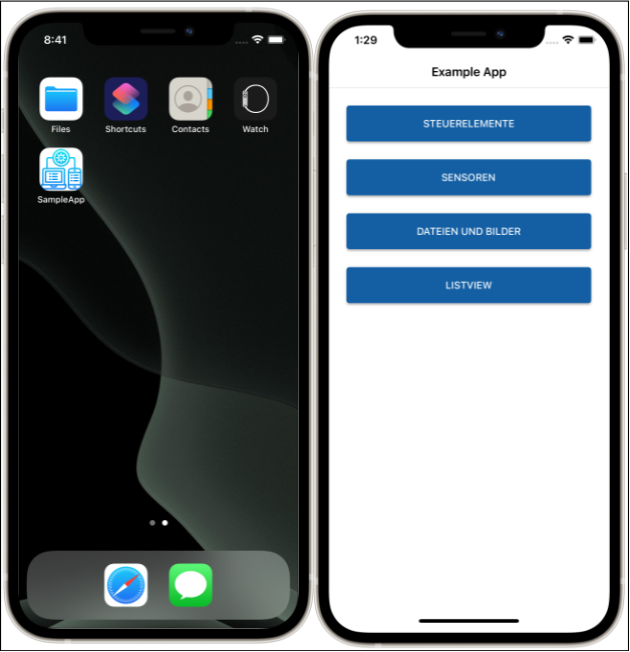
\includegraphics[width=\textwidth,keepaspectratio]{Images/Screenshot/AppIconAndMenu.png}
 \caption{Test Objekt Screenshots I}
 \label{fig:TestObjectI}
\end{figure}

Über dieses Menu kann der Anwender zu verschiedenen Seiten navigieren, die folgend kurz erläutert werden sollen.  Die in Abbildung \ref{fig:TestObjectII} zeigt die Seite mit den verfügbaren Steuerelementen von Xamarin.Forms,  wie sie auch in Kapitel 3 beschrieben wurden. Dazu gehören Ansichten für die Präsentation, für Interaktionen, zum setzen von Werten, für die Manipulation von Texten und für die Anzeige von aktuellen Interaktionen.
\begin{figure}[!ht]
 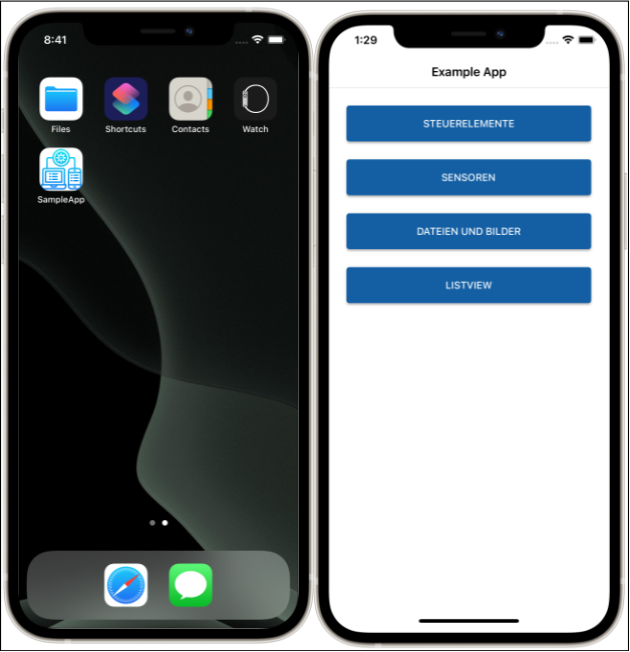
\includegraphics[width=\textwidth,keepaspectratio]{Images/Screenshot/AppIconAndMenu.png}
 \caption{Test Objekt Screenshots II}
 \label{fig:TestObjectII}
\end{figure}

Die folgende Option Sensoren öffnet eine Ansicht, auf der die aktuellen Werte von den Smartphone-Sensoren ausgegeben werden.  Diese Sensoren werden von vielen mobilen Anwendungen verwendet. Dazu gehören der Beschleunigungssensor, der Compass,  das Gyroscope und das Magnetometer.  Anhand dieser Seite,  soll sichergestellt werden, dass der Compiler auch die Funktionalität dieser Sensoren Abbilden kann. 

\begin{figure}[!ht]
 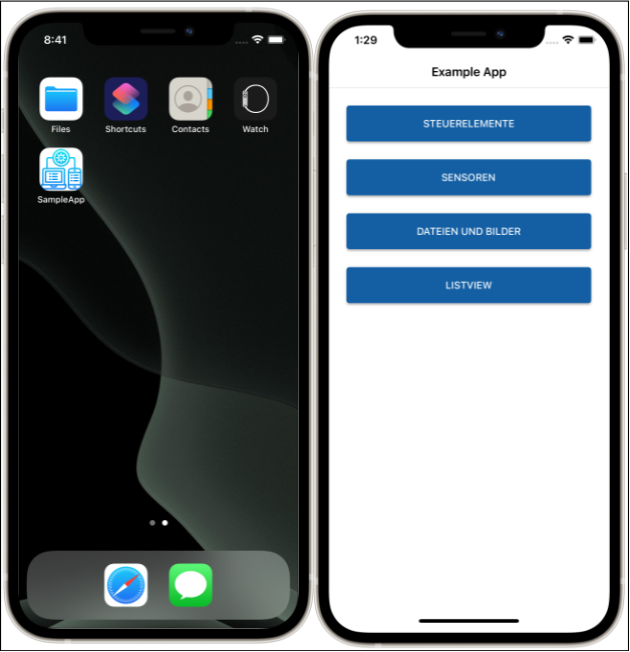
\includegraphics[width=\textwidth,keepaspectratio]{Images/Screenshot/AppIconAndMenu.png}
 \caption{Test Objekt Screenshots III}
 \label{fig:TestObjectIII}
\end{figure}

Ebenfalls werden in dem Testprojekt eine Liste und ein Carousel abgebildet,  da es sich bei diesen um häufig verwendete Elemente handelt - die in vielen mobilen Anwendungen verwendet wird. 

\begin{figure}[!ht]
 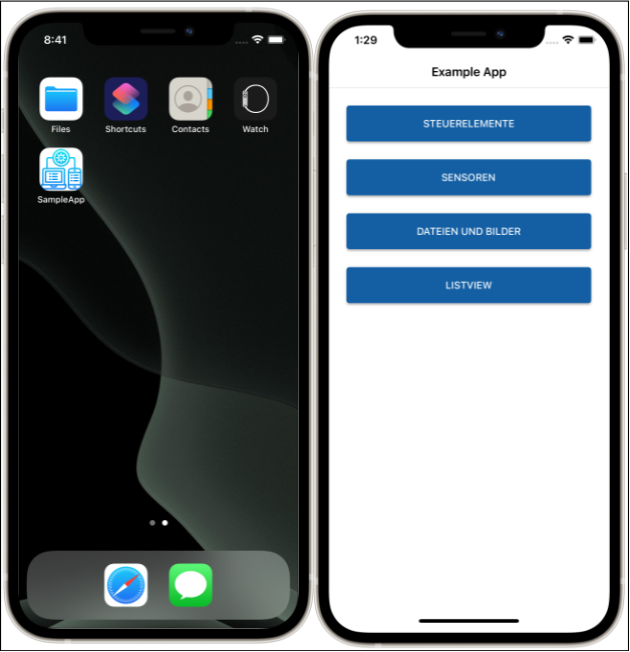
\includegraphics[width=\textwidth,keepaspectratio]{Images/Screenshot/AppIconAndMenu.png}
 \caption{Test Objekt Screenshots IV}
 \label{fig:TestObjectIV}
\end{figure}




\section{Testablauf}




\section{Testauswertung}



  \chapter{Fazit und Ausblick}
\label{chap:FazitAusblick}

Flutter immernoch eine Abhängigkeit
  
  \appendix                       % Leitet den Nachspann ein
  \addtocontents{toc}{\protect\renewcommand*{\protect\@pnumwidth}{3em}}
    \renewcommand*\chapterheadstartvskip{}% removes space before chapter titles 

  \renewcommand*{\chapterpagestyle}{scrheadings}

\setlength\bibitemsep{1.5\itemsep}
\chapter*{Literaturverzeichnis}
\pagenumbering{Roman}
\setcounter{page}{11}
 \chaptermark{Literaturverzeichnis}

 \addcontentsline{toc}{chapter}{Literaturverzeichnis}

\printbibliography[nottype=online, heading=subbibliography, title={Gedruckte Quellen}]
\printbibliography[type=online, heading=subbibliography, title={Online Quellen}]
  \include{AnhangGegenüberstellung}
  \chapter{Anhang II: Optimierte Flutter-LoginPage}
\label{chap:OptimizedLoginPage}


\lstinputlisting[caption={[]{Optimierte Flutter-LoginPage}} , language=Dart]{SourceCode/FlutterLoginPageUpdate.Dart} 

  \chapter{Anhang III: Android Screenshots}
\label{chap:AnhangAndroidScreenshots}

\begin{figure}[!ht]
 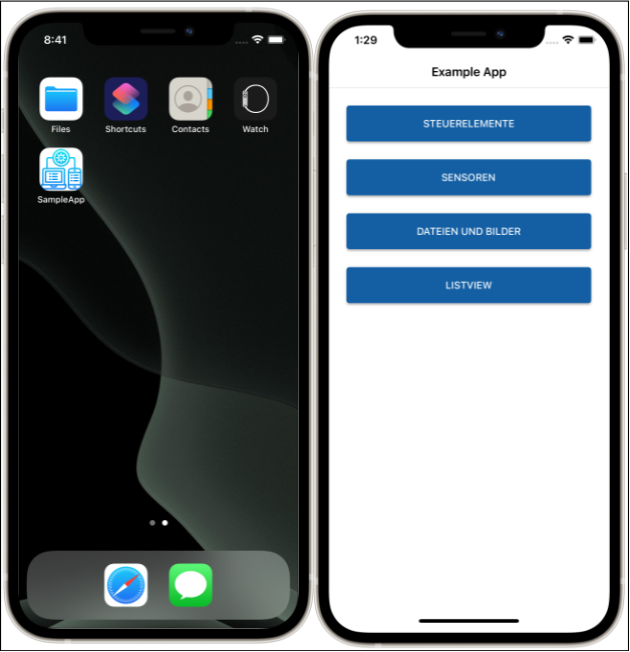
\includegraphics[width=\textwidth,keepaspectratio]{Images/Screenshot/AppIconAndMenu.png}
 \caption[]{Test Objekt Screenshots I}
\end{figure}

\begin{figure}[!ht]
 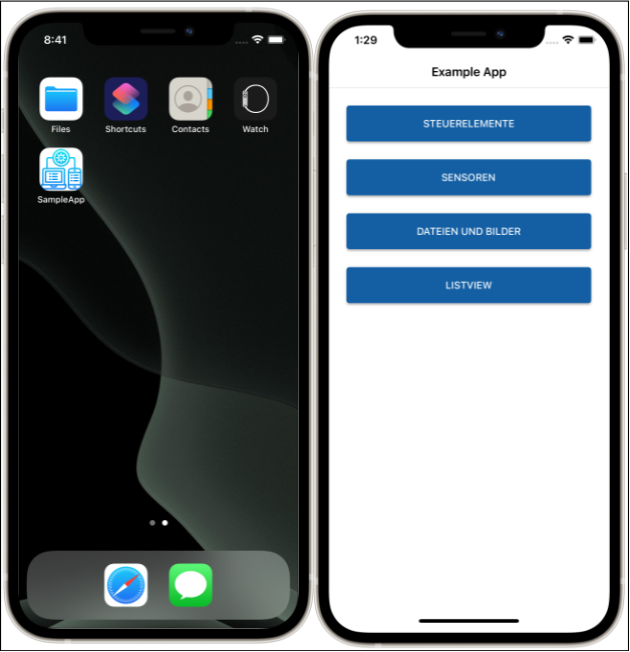
\includegraphics[width=\textwidth,keepaspectratio]{Images/Screenshot/AppIconAndMenu.png}
 \caption[]{Test Objekt Screenshots II}
\end{figure}

\begin{figure}[!ht]
 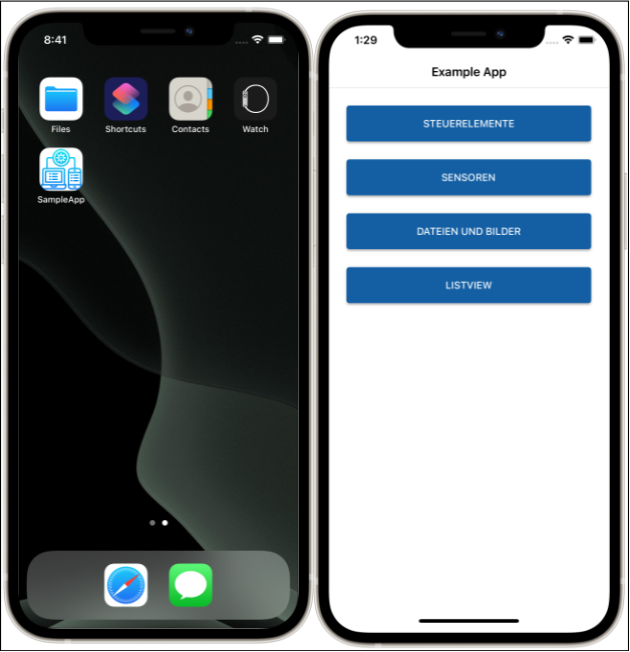
\includegraphics[width=\textwidth,keepaspectratio]{Images/Screenshot/AppIconAndMenu.png}
 \caption[]{Test Objekt Screenshots III}
\end{figure}

\begin{figure}[!ht]
 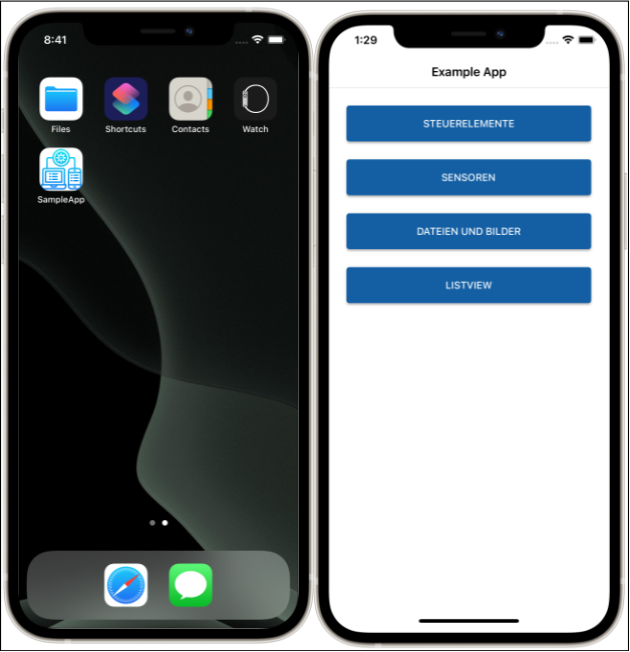
\includegraphics[width=\textwidth,keepaspectratio]{Images/Screenshot/AppIconAndMenu.png}
 \caption[]{Test Objekt Screenshots IV}
\end{figure}



  \chapter{Anhang IV: Android Screenshots der Flutter App}
\label{chap:AnhangAndroidScreenshotsFlutter}


\begin{figure}[ht!]
 \includegraphics[width=\textwidth,keepaspectratio]{Images/Screenshot/AndroidScrenshotI.png}
\end{figure}

\newpage
\begin{figure}[ht!]
 \includegraphics[width=\textwidth,keepaspectratio]{Images/Screenshot/AndroidScreenshot2.png}
\end{figure}

  \chapter{Anhang V: Installationsanleitung}
\label{chap:Installationsanleitung}




  \printEidesstattlicheErklaerung % Setzt die eidesstattlichen Erklärung
\end{document}
